\documentclass[12pt, a4paper, twoside]{report}
\newcommand\student{Nguyễn Trí Hiếu}
\newcommand\mssv{1711298}
\newcommand\thesisname{Ứng dụng neural networks vào giải điều chế tín hiệu trong hệ thống VLC}
\newcommand\reportname{Luận văn tốt nghiệp}
\newcommand\supervisor{TS. Phạm Quang Thái}
\newcommand\ngaygiaonhiemvu{22-1-2020}
\newcommand\ngayxongnhiemvu{1-7-2021}
\newcommand\noidungnhiemvu{
	\begin{itemize}\setlength\itemsep{-0.2em}
	\item Đo đạc trên hệ thống VLC tại phòng thí nghiệm 209B1
	\item Giải điều chế tín hiệu sử dụng neural networks
	\end{itemize}
}
\usepackage[utf8]{vietnam}
\usepackage{indentfirst} 
\usepackage{amsmath, amsfonts, amssymb}
\usepackage{graphicx}
\usepackage{multicol}
\usepackage{caption}
\usepackage{geometry}
\usepackage{cite}
\usepackage{subcaption}
\usepackage{titlesec} 
\usepackage{acro}
\usepackage{listings}
\usepackage{fancyhdr}
\usepackage{tikz}
\usepackage{slashbox}
\usepackage{float}
\usepackage{hyperref}
\usepackage{multirow}
\def\BibTeX{{\rm B\kern-.05em{\sc i\kern-.025em b}\kern-.08em
    T\kern-.1667em\lower.7ex\hbox{E}\kern-.125emX}}
\usetikzlibrary{shapes.geometric, arrows}
\tikzstyle{startstop} = [rectangle, rounded corners, minimum width=2.5cm, minimum height=0.75cm,text centered, draw=black]
\tikzstyle{io} = [trapezium, trapezium left angle=70, trapezium right angle=110, minimum width=2.5cm, minimum height=0.75cm, text centered, draw=black, text width=2cm]
\tikzstyle{process} = [rectangle, minimum width=2.5cm, minimum height=0.75cm, text centered, draw=black, text width=3cm]
\tikzstyle{decision} = [diamond, minimum width=2cm, minimum height=2cm, text centered, draw=black, text width=1cm]
\tikzstyle{arrow} = [thick,->,>=stealth]
\geometry{
	a4paper,
	total={160mm,247mm},
	left=25mm,
	right=25mm,
	top=25mm,
	bottom=25mm,
}
\definecolor{codegreen}{rgb}{0,0.6,0}
\definecolor{codegray}{rgb}{0.5,0.5,0.5}
\definecolor{codepurple}{rgb}{0.58,0,0.82}
\definecolor{backcolour}{rgb}{0.95,0.95,0.92}

\lstdefinestyle{mystyle}{
    backgroundcolor=\color{backcolour},   
    commentstyle=\color{codegreen},
    keywordstyle=\color{magenta},
    numberstyle=\tiny\color{codegray},
    stringstyle=\color{codepurple},
    basicstyle=\ttfamily\footnotesize,
    breakatwhitespace=false,         
    breaklines=true,                 
    captionpos=b,                    
    keepspaces=true,                 
    numbers=left,                    
    numbersep=5pt,                  
    showspaces=false,                
    showstringspaces=false,
    showtabs=false,                  
    tabsize=2
}

\lstset{style=mystyle}
\def\coverpage
	{
	\pagestyle{empty} 
	 	\begin{minipage}[b][25.5cm][t]{15cm}	
		\begin{center}
		{
		\vspace{3cm}
		\fontsize{20}{1}\selectfont 
		\textbf{\parbox[c][3cm]{14cm}{\centering \MakeUppercase{\thesisname}}
		}
		\\
		\vspace{0.1\paperheight}
		{\fontsize{14}{1}\selectfont 
		\MakeUppercase{\reportname}
		\\
		\vspace{0.05\paperheight}
		\student \space -- \mssv
		\\
		Giảng viên hướng dẫn
		\\
		\supervisor
		}
		}
		\\
		\vspace{0.25\paperheight}
		\begin{minipage}{0.8\textwidth}
			\begin{minipage}{0.2\textwidth}
				
\includegraphics[width=0.7\linewidth]{Image/logo}
			\end{minipage}
			\begin{minipage}{\textwidth}\centering \raggedright
				{\fontsize{12}{1}\selectfont
				ĐẠI HỌC QUỐC GIA THÀNH PHỐ HỒ CHÍ MINH\\
				TRƯỜNG ĐẠI HỌC BÁCH KHOA\\
				KHOA ĐIỆN – ĐIỆN TỬ, BỘ MÔN VIỄN THÔNG\\
				}
			\end{minipage}
		\end{minipage}
		\\
		\vspace{0.05\paperheight}
		\the\month\space -- \the\year	
		\end{center}		
	\end{minipage}
	}
\def\nhiemvuluanvanpage	
{
	\cleardoublepage
	\begin{minipage}{0.5\textwidth}
		\begin{center}
			{\fontsize{9}{1}\selectfont
			ĐẠI HỌC QUỐC GIA THÀNH PHỐ HỒ CHÍ MINH\\
			TRƯỜNG ĐẠI HỌC BÁCH KHOA\\}
		\end{center}
	\end{minipage}
	\begin{minipage}{0.5\textwidth}
		\small
		\begin{center}
			{\fontsize{9}{1}\selectfont
			CỘNG HÒA XÃ HỘI CHỦ NGHĨA VIỆT NAM\\
			Độc lập -- Tự do -- Hạnh Phúc\\}
		\end{center}
	\end{minipage}
	\begin{center}
		\underline{\hspace{0.8\textwidth}}
	\end{center}

	\begin{minipage}{0.8\textwidth}
		Số:\underline{\hspace{2.4cm}}/BKĐT\\
		Khoa: \textbf{Điện -- Điện tử}\\
		Bộ môn: \textbf{Viễn thông}
	\end{minipage}
	\begin{center}
		\bfseries{\MakeUppercase{Nhiệm vụ luận văn tốt nghiệp}}
	\end{center}
	\begin{enumerate}\setlength\itemsep{-0.2em}
	\item 
	\begin{tabbing}
	Họ và tên: \= \student, \hspace{0.15\paperwidth} \= MSSV: \mssv
	\end{tabbing}
	\item Ngành: Điện -- Điện tử, Chuyên ngành: Kỹ thuật Điện tử -- Truyền thông
	\item Đề tài: \thesisname
	\item Nhiệm vụ: \noidungnhiemvu
	\item Ngày giao nhiệm vụ: \ngaygiaonhiemvu
	\item Ngày hoàn thành nhiệm vụ: \ngayxongnhiemvu
	\item 
	\begin{tabbing}
	Họ và tên người hướng dẫn: \hspace{0.25\paperwidth} \=  Phần hướng dẫn:\\
	\supervisor \> 100\%\\
	BM Viễn Thông, Khoa Điện – Điện Tử
	\end{tabbing}
	\end{enumerate}
	
	Nội dung và yêu cầu LVTN đã được thông qua Bộ Môn.
	
	\vspace{\baselineskip}
	\begin{minipage}{0.5\textwidth}
		\begin{center}
			{\fontsize{12}{1}\selectfont
			Tp. HCM, Ngày \underline{\hspace{0.5cm}} tháng \underline{\hspace{0.5cm}} năm 20\underline{\hspace{0.5cm}} \\
			\textbf{CHỦ NHIỆM BỘ MÔN}\\
			\par
			\vspace{0.06\paperheight}	
			PGS. TS. Hà Hoàng Kha
			}
		\end{center}
	\end{minipage}	
	\begin{minipage}{0.5\textwidth}
		\begin{center}
			{\fontsize{12}{1}\selectfont
			Tp. HCM, Ngày \underline{\hspace{0.5cm}} tháng \underline{\hspace{0.5cm}} năm 20\underline{\hspace{0.5cm}} \\
			\textbf{NGƯỜI HƯỚNG DẪN CHÍNH}\\
			\vspace{0.06\paperheight}	
			\supervisor
			}
		\end{center}
	\end{minipage}
	
	\vspace{\baselineskip}
	\begin{minipage}{0.8\textwidth}
		\textbf{PHẦN DÀNH CHO KHOA, BỘ MÔN:}\\
		Người duyệt (chấm sơ bộ): \underline{\hspace{3.5cm}} \\
		Đơn vị:\underline{\hspace{7.1cm}} \\
		Ngày bảo vệ:\underline{\hspace{6.1cm}}\\
		Điểm tổng kết:\underline{\hspace{5.75cm}}\\
		Nơi lưu trữ luận văn:\underline{\hspace{4.65cm}}\\
	\end{minipage}
}
\DeclareAcronym{ber}{
short = BER,
long = Bit Error Rate
}
\DeclareAcronym{rf}{
short = RF,
long = Radio Frequency
}
\DeclareAcronym{snr}{
short = SNR,
long =Signal to Noise Ratio
}
\DeclareAcronym{vlc}{
short = VLC, 
long = Visible Light Communication
}
\DeclareAcronym{owc}{
short = OWC, 
long = Optical Wireless Communication
}
\DeclareAcronym{ofdm}{
short = OFDM, 
long = Orthogonal Frequency Division Multiplexing
}
\DeclareAcronym{m-pam}{
short = M-PAM, 
long = M-ary Pulse Amplitude Modulation
}
\DeclareAcronym{ann}{
short = ANN, 
long = Artificial Neural Networks
}
\DeclareAcronym{dnn}{
short = DNN, 
long = Deep Neural Networks
}
\DeclareAcronym{cnn}{
short = CNN, 
long =Convolutional Neural Networks
}
\DeclareAcronym{ook}{
short = OOK, 
long = On Off Keying
}
\DeclareAcronym{led}{
short = LED, 
long = Light Emitting Diode
}
\DeclareAcronym{oled}{
short = OLED, 
long = Organic Light Emitting Diode
}
\DeclareAcronym{dsp}{
short = DSP, 
long = Digital Signal Processing
}
\DeclareAcronym{isi}{
short = ISI, 
long = Intersymbol Interference
}
\DeclareAcronym{los}{
short = LOS, 
long = Light of sight
}
\DeclareAcronym{nlos}{
short = NLOS,
long = Non light of sight
}
\DeclareAcronym{cce}{
short = CCE,
long = Categorical Cross Entropy
}
\DeclareAcronym{samme}{
short = SAMME,
long = Stagewise Additive Modeling using a Multi-class Exponential loss function
}
\DeclareAcronym{ask}{
short = ASK,
long = Amplitude Shift Keying
}
\DeclareAcronym{awgn}{
short = AWGN,
long = Additive White Gaussian Noise
}
\DeclareAcronym{m2m}{
short = M2M, 
long = Machine to Machine
}
\DeclareAcronym{cap}{
short = CAP, 
long = carrier-less amplitude and phase
}
\DeclareAcronym{fft}{
short = FFT, 
long = fast Fourier transform
}
\DeclareAcronym{pnn}{
short = PNN, 
long = Probabilistic Neural Networks
}
\DeclareAcronym{pdf}{
short = PDF, 
long = hàm mật độ xác suất
}
\DeclareAcronym{grnn}{
short = GRNN, 
long = General Regression Neural Networks
}
\DeclareAcronym{mse}{
short = MSE, 
long = Mean Squared Error
}
\DeclareAcronym{ae}{
short = AE, 
long = Autoencoder
}
\DeclareAcronym{nrz}{
short = NRZ, 
long = Non return to zero
}
\DeclareAcronym{vppm}{
short = VPPM, 
long = Variable Pulse Position Modulation
}
\DeclareAcronym{csk}{
short = CSK, 
long = Color Shift Keying
}
\DeclareAcronym{gan}{
short = GAN, 
long = Generative adversarial networks
}
\DeclareAcronym{dae}{
short = DAE, 
long = Denoising Autoencoder
}
\DeclareAcronym{ssl}{
short = SSL, 
long = Solid State Lighting
}
\DeclareAcronym{pled}{
short = PLED, 
long = Polymer Light Emitting Diode
}
\DeclareAcronym{cwt}{
short = CWT, 
long = Continuous wavelet transform
}
\DeclareAcronym{dtnn}{
short = DTNN, 
long = Deep Tensor Neural Networks
}
\DeclareAcronym{wlan}{
short = WLAN, 
long = Wireless local area networks
}
\DeclareAcronym{lstm}{
short = LSTM, 
long = Long Short Term Memory
}


\begin{document}

\coverpage

\nhiemvuluanvanpage

\titleformat{\chapter}
  {\Large\bfseries}
  {\thechapter .}
  {.5em}
  {\filleft\MakeUppercase}
  [\vspace{.5ex}]
\chapter*{Lời cám ơn}
	Để hoàn thành báo cáo này, em xin chân thành gửi lời cảm ơn đến:

Đầu tiên và sâu sắc nhất là thầy TS. Phạm Quang Thái, người đã giúp đỡ em xuyên suốt trong quá trình hoàn thành luận văn tốt nghiệp. Từ những ngày đầu tiên, khi em gặp khó khăn, thầy đã sẵn sàng góp ý, tận tình giúp đỡ, chỉ ra những điểm thiếu sót, gợi ý phương pháp làm bài, nguồn tài liệu, …Đó là những đóng góp quý báu giúp em có thể hoàn thành báo cáo.

Kế đến cũng không thể không nhắc đến công lao của quý thầy cô khoa Điện-điện tử, đại học Bách Khoa thành phố Hồ Chí Minh, những người đã chỉ dạy em trong những năm vừa qua.

Cuối cùng, xin gửi lời cảm ơn đến các bạn, các anh cùng học tập, nghiên cứu tại phòng thí nghiệm 209B1.

Xin chúc những điều tốt đẹp nhất sẽ luôn đồng hành cùng quý thầy cô và các bạn.

	\vspace{\baselineskip}
	\hfill
	\begin{minipage}{0.5\textwidth}
		\begin{center}
			{\fontsize{12}{1}\selectfont
			Tp. HCM, \today 
			\vspace{0.1\paperheight}	
			\student
			}
		\end{center}
	\end{minipage}
\chapter*{Lời cam đoan}
	Tôi tên: \student \space (MSSV: \mssv), 
	là sinh viên chuyên ngành Kỹ thuật Điện tử - Truyền thông, tại Trường Đại học Bách Khoa, Đại học Quốc gia thành phố Hồ Chí Minh. Tôi xin cam đoan những nội dung sau đều là sự thật: 	
	\begin{itemize}
		\item  Công trình nghiên cứu này hoàn toàn do chính tôi thực hiện; 
		\item  Các tài liệu và trích dẫn trong báo cáo này được tham khảo từ các nguồn thực tế, có uy tín và độ chính xác cao; 
		\item  Các số liệu và kết quả của công trình này được tôi tự thực hiện một cách độc lập và trung thực.
	\end{itemize}

	\vspace{\baselineskip}
	\hfill
	\begin{minipage}{0.5\textwidth}
		\begin{center}
			{\fontsize{12}{1}\selectfont
			Tp. HCM, \today 
			\vspace{0.1\paperheight}	
			\student
			}
		\end{center}
	\end{minipage}
\chapter*{Tóm tắt nội dung}
	Trong luận văn này bao gồm hai phần chính là đo đạc tại phòng thí nghiệm 209B1 (Hcmut) và xây dựng những mô hình học máy khác nhau để giải điều chế tín hiệu. Dữ liệu từ việc đo đạc tín hiệu 2 mức xung Lorentz trên hệ thống truyền thông bằng ánh sáng khả kiến dùng \ac{oled} được sử dụng làm tập dữ liệu cho mô hình máy học. Luận văn này sẽ trình chi tiết các quá trình từ đo đạt dữ liệu,  xử lý tín hiệu đến phân loại tín hiệu.

Các bước xử lý tín hiệu sẽ khảo sát bao gồm: giảm méo dạng phi tuyến bằng Denoising Autoencoder Neural Networks. Dữ liệu để huấn luyện là tín hiệu 2 mức ngẫu nhiên được cộng thêm nhiễu Gaussian. Mục tiêu của mô hình là học được những đặc tính của tín hiệu 2 mức, để có thể hiệu chỉnh lại tín hiệu bị méo dạng khi đi qua kênh truyền \ac{vlc}. Cách thứ 2 được khảo sát là trích xuất tín hiệu thành từng frame, mỗi frame sẽ bao gồm bit cần phân loại cùng với hai bits liền trước và hai bits liền sau nó. Ngoài ra, do tín hiệu thu được là nonstationary, nên một kỹ thuật phân tín tín hiệu trong cả miền thời gian và tần số là \ac{cwt} cũng được sử dụng.

Để có thể phân loại tín hiệu với 2 mức khác nhau, chúng tôi sẽ sử dụng 3 phương pháp là \ac{pnn}, \ac{grnn} và \ac{dtnn}, sau đó sẽ so sánh 3 phương pháp với nhau và với phương pháp thông thường là bộ giải điều chế dùng ngưỡng.

Mục tiêu của luận văn này là đi tìm phương pháp tiền xử lý cũng như phân loại tín hiệu tốt nhất để có thể làm giảm \ac{ber} xuống mức dưới ngưỡng cho phép trong hệ thống \ac{vlc} là 3.8e - 3, với tốc độ bit và khoảng cách cao nhất có thể. 

\chapter*{Abstract}
	In this thesis, the two main parts are: measuring at laboratory 209B1 (Hcmut) and building different machine learning models for signal demodulation. Data from the measurement of two Lorentz pulses signals on visible light communication systems using \ac{oled} use as datasets for the machine learning model. This thesis will detail the processes from data acquisition, signal processing to signal classification. 

The signal processing steps to be investigated include: reducing nonlinear distortion with Denoising Autoencoder Neural Networks. The data to train is a 2-level randomized pulse with added Gaussian noise. The goal of the model is to learn the characteristics of a two-level pulse to correct the distorted signal when passing through the \ac {vlc} channel. The second way to be investigated is to extract the signal into frames. Each frame contains the classified bit along with the two preceding and two bits following it. In addition, since the received signal is nonstationary, a time domain and frequency domain \ac{cwt} technique is also used. 

To be able to classify signals with two different levels, we will use three methods: \ac{pnn}, \ac{grnn} and \ac{dtnn}, then compare the three methods with each other and with the demodulator using a threshold. 

The goal of this thesis is to find the best method of preprocessing as well as classifying signals that can reduce \ac{ber} to a level below the allowable threshold in the \ ac {vlc} system of 3.8e - 3, with the highest possible bit rate and distance. 
\tableofcontents
{%
 \let\oldnumberline\numberline%
 \renewcommand{\numberline}{\figurename~\oldnumberline}%
 \listoffigures%
}
{%
\let\oldnumberline\numberline%
\renewcommand{\numberline}{\tablename~\oldnumberline}%
\listoftables%
}
\printacronyms[name = {Danh sách từ viết tắt}]

\fancyhead{}  % Clears all page headers and footers
\fancyhead[L]{\nouppercase\leftmark}
\fancyhead[R]{\thepage}
\cfoot{}
\pagestyle{fancy}

\titleformat{\chapter}
  {\Large\bfseries}
  {Chương \thechapter .}
  {.5em}
  {\filleft\MakeUppercase}
  [\vspace{.5ex}]
\chapter{GIỚI THIỆU} \label{sec:chapter_1}
\section{Đặt vấn đề}
Sự giới hạn của phổ tần số là hạn chế của cho việc tăng độ phổ biến và dung lượng kênh truyền. Theo CISCO \cite{cisco}, số lượng thiết bị kết nối vào mạng IP sẽ nhiều hơn gấp 3 lần dân số thế giới vào năm 2023. Cụ thể, sẽ có trung bình 3.6 thiết bị trên một người năm 2023, so với 2.4 thiết bị trên một người 2018. Kết nối \ac{m2m} sẽ chiếm một nửa các kết nối trên toàn cầu vào năm 2023 (tăng từ 33 \% năm 2018 lên 50 \% vào năm 2023), và sẽ có 14.7 tỷ kết nối \ac{m2m} vào năm 2023. Hơn 70 \% dân số thế giới có thiết bị kết nối di động năm 2023. Lưu lượng di động trung bình của một người trên một tháng tăng gấp 6 lần từ năm 2017 đến năm 2022.
Sự tăng số lượng các thiết bị và nhu cầu sử dụng là nguyên nhân chính cho việc tăng lưu lượng dữ lượng di động. 
\begin{figure} [ht]
\centering
\captionsetup{justification=centering}
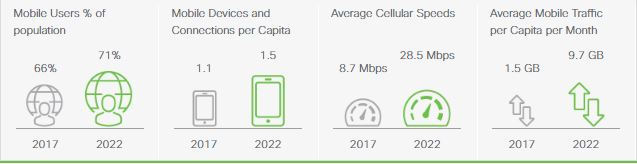
\includegraphics [scale=0.9] {Image/cisco_forecast}
\caption{Dự đoán của Cisco về dữ liệu di động \cite{cisco_forecast}}
\end{figure}
Mặc dù các nhà cung cấp dịch vụ không dây đang triển khai thêm cơ sở hạ tầng bằng cách bổ sung những trạm phát Wi-fi, nhưng hạn chế là việc sử dụng quá mức phổ \ac{rf} hiện có. Từ đó gây ra can nhiễu và chồng lấn phổ làm tăng độ trễ và giảm dung lượng. Để khắc phục tình trạng trên, một công nghệ mới đã và đang được phát triển đó là \ac{vlc} ứng dụng trong \ac{ssl} hoặc công nghệ hiển thị độ phân giải cao. Mặc dù hệ thống \ac{vlc} dùng \ac{led} chiếm tỷ lệ vượt trội khi hỗ trợ tốc độ dữ liệu cao, giá rẻ, ... Tuy nhiên với sự phát triển vượt bậc trong nhưng năm gần đây, cùng với những ưu điểm như như màu sắc dễ chịu, khả năng kiểm soát màu sắc tốt, diện tích phát xạ lớn, ...\ac{oled} được kỳ vọng sẽ trở thành công nghệ phát sáng quan trọng trong tương lai.

Hiện nay, trong các hệ thống thông tin quang \ac{vlc} đa phần dùng kiểu điều chế \ac{ofdm}.  Việc điều chế bằng \ac{ofdm} có ưu điểm là giúp cho băng thông của tín hiệu tiết kiệm được rất nhiều. Nếu dùng \ac{led} đơn có thể đạt đến 3Gbps cho khoảng băng thông khoảng 380Mhz tương ứng với 7.89bits/s/Hz trong khoảng cách 5cm, và khoảng 80Mbits/s trong 20Mhz tương ứng 4bits/s/Hz trong khoảng cách 1m. Nhưng có một khuyết điểm là \ac{ofdm} xử lý tín hiệu phức tạp trong miền \ac{dsp}, vì ngoài việc xử lý qua nhiều giai đoạn, \ac{ofdm} rất dễ nhạy cảm với việc trôi tần số nên ta cần các thuật toán và phần cứng để đồng bộ bước sóng quang và tần số phần điện. Vì vậy, ngoài việc tiếp cận bằng \ac{ofdm} thì có nhiều cách tiếp cận khác để nâng hiệu quả sử dụng băng thông, trong đó có phương pháp điều chế \ac{ook} sử dụng mã đường truyền \ac{nrz}.

Do đó, đề tài nghiên cứu việc ứng dụng neural network vào giải điều chế tín hiệu \ac{nrz} trong hệ thống \ac{vlc} dùng \ac{oled}. 

Câu hỏi nghiên cứu đặt ra của luận văn là: 
\begin{itemize}
\item Phương pháp neural network có tốt hơn phương pháp giải điều chế truyền thống hay không?
\item Mô hình và thông số nào của neural network phù hợp nhất cho việc giải điều chế?
\item Mô hình và phương pháp nào là cách tốt nhất cho việc tiền xử lý dữ liệu.
\end{itemize} 

Trong chương \ref{sec:chapter_2}, cơ sở lý thuyết về hệ thống \ac{vlc}, neural network và các phương pháp tiền xử lý sẽ được trình bày. Trong chương \ref{sec:chapter_3}, các kết quả đo đạc và giải điều chế sẽ được so sánh và phân tích. Cuối cùng, chương \ref{sec:chapter_4} đưa ra kết luận chung.

\section{Phạm vi và phương pháp nghiên cứu}
\begin{itemize}
\item Phạm vi: thử nghiệm việc giải điều chế \ac{nrz} dùng 3 phương pháp neural networks.
\item Phương pháp nghiên cứu: đo đạc tại lab 209B1, với hệ thống quang không dây dùng \ac{oled}. Các phương pháp để tiền xử lý dữ liệu gồm có \ac{cwt}, framing, \ac{dae}. Các phương pháp sử dụng để giải điều chế là \ac{pnn}, \ac{grnn}, \ac{dtnn}.
\end{itemize}
\section{Các đóng góp}
\begin{itemize}
\item Đo đạc tín hiệu \ac{nrz} và xung lorentz trên hệ thống \ac{vlc} dùng \ac{oled}, tính toán \ac{snr}, \ac{ber} và xử lý dữ liệu thu được từ osciloscope để đưa vào mô hình phân loại.
\item Xây dựng thành công các mô hình neural network cho phép phân loại các mức tín hiệu \ac{nrz} và xung lorentz và so sánh của những mô hình trên.
\item Nghiên cứu những phương pháp tiền xử lý để gia tăng độ chính xác cho mô hình phân loại.
\end{itemize}
\chapter{CƠ SỞ LÝ THUYẾT}\label{sec:chapter_2}
\section{Tổng quan về hệ thống VLC}

\subsection{Giới thiệu}
Hệ thống \ac{vlc} sử dụng ánh sáng khả kiến có tần số từ 400 - 800 THz (780–375 nm), có ưu điểm về hiệu quả trong việc sử dụng vùng quang phổ cao, vùng băng thông rộng không cần giấy phép và độ an toàn cao. Khi so sánh với công nghệ truyền thông chủ yếu được sự dụng ở thời điểm hiện tại là \ac{rf}, \ac{vlc} có một số ưu điểm như: 
\begin{itemize}
\item Thứ nhất \ac{vlc} có băng thông tầng số gấp nhiều lần so với băng thông của \ac{rf} (300 THz của \ac{vlc} và 300 Ghz của \ac{rf}). Trong \ac{rf} vùng phổ không cần giấy phép là từ 57-66 GHz ở vùng băng thông siêu cao tần. Nó vẫn nhỏ hơn là vùng phổ so với \ac{vlc}, vì ở \ac{vlc} thì không cần giấy phép và có thể sử dụng miễn phí. Điều đó có nghĩa là \ac{vlc} có thể hỗ trợ tốc độ dữ liệu cao và có thể sử dụng lại băng thông.   
\item Thứ hai, \ac{vlc} có thể an toàn hơn so với \ac{rf}. Nó không thể xuyên qua tường và các vật thể trong suốt khác trong điều kiện trong nhà. Điều đó có nghĩa là thông tin truyền đi của người sử dụng sẽ được giới hạn trong phòng. Vì vậy, an toàn thông tin có thể được đảm bảo. 
\end{itemize}

Ví dụ \cite{rf-vs-vlc}, trong hình \ref{fig:rf-vs-vlc} chỉ ra cách hệ thống \ac{vlc} có thể sử dụng lại quang phổ một cách hiệu quả trong vùng không gian nhỏ. Trường hợp a) chỉ ra rằng kênh truyền WiFi trong đó ba người dùng chia sẽ nhau băng thông 30 Mb/s với trường hợp b) mỗi user sử dụng riêng 10 Mb/s trên kênh truyền \ac{vlc}. Mặc dù tổng băng thông sử dụng trong hai trường hợp là như nhau nhưng trường hợp b) tốt hơn vì hiệu ứng chồng lấn phổ trên kênh truyền \ac{rf}.

\begin{figure} [ht]
\centering
\captionsetup{justification=centering}
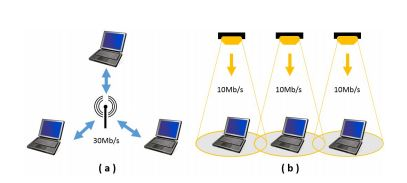
\includegraphics [scale=1] {Image/rf_vs_vlc}
\caption{So sánh băng thông sử dụng của RF và VLC}
\label{fig:rf-vs-vlc}
\end{figure}

\subsection{Kỹ thuật điều chế \cite{VLC-application}}
Khác với điều chế trong giao tiếp RF vì sự không mã hóa đặc trưng thông tin thành pha và biên độ của tín hiệu ánh sáng. Hệ thống mã hóa trong VLC được thực hiện dựa trên cường độ của sóng ánh sáng. Giải điều chế bằng cách phát hiện trực tiếp dựa trên tín hiệu thu được. Có hai vấn đề chính được xem xét trong việc thiết kế hệ thống điều chế cho \ac{vlc} gồm:
\begin{itemize}
	\item Dimming: những hoạt động khác nhau yêu cầu độ sáng khác nhau. Như là 30-100 lux yêu cầu cho những hoạt động thị giác thông thường tại nơi công cộng, tuy nhiên có những ứng dụng dành cho văn phòng hay nhà ở cần đến 300 - 1000 lux. Mối quan hệ không tuyến tính của ánh sáng đo đạc (measured light) và ánh sáng cảm nhận được (perceived light) được cho bởi:
\begin{equation}
Perceived \, light (\%) = 100 \times \sqrt{\frac{Measured \, light (\%)}{100}}
\end{equation}
	\item Flickering: sự thay đổi về độ sáng của ánh sáng điều chế nên được thực hiện theo cách để con người không nhận ra được sự biến đổi. Theo tiêu chuẩn IEEE 802.15.7, dao động của cường độ ánh sáng nên lớn hơn 200 Hz để tránh những tác động có hại cho mắt.
\end{itemize}

Những phương pháp điều chế thường được sử dụng như:
\begin{itemize}
\item \ac{ook}
\item Pulse Modulation
\item \ac{ofdm}
\item \ac{csk}
\end{itemize}
\begin{table}[H]
	\caption{Bảng so sánh các phương pháp điều chế trong VLC}.
	\begin{center}
	\small
		\begin{tabular}{|c|c|c|c|}
			\hline
			Phương pháp điều chế & \ac{ber} & \ac{snr} (dB) & Data rate\\
			\hline
    			PWM
			&Cao			
			&Thấp
			&Thấp nhất\\
			\hline
    			PPM
			&Cao			
			&Trung bình
			&Thấp\\
			\hline
    			\ac{csk}
			&Thấp hơn			
			&Trung bình
			&Trung bình\\
			\hline
			\ac{ook}
			&Thấp nhất			
			&Cao
			&Trung bình\\
			\hline
			MIMO OFDM
			&Cao			
			&Thấp
			&Cao nhất\\
			\hline
		\end{tabular}
		\label{tab: so-sanh-mod}
	\end{center}
\end{table}

Tiêu chuẩn IEEE 802.15.7 định nghĩa 3 loại lớp vật lý trong hệ thống \ac{vlc}, được phân loại theo tốc độ dữ liệu. PHY I có tốc độ dữ liệu từ 11.67 kb/s đến 266.7 kb/s, PHY II từ 1.25 Mb/s đến 96 Mb/s, PHY III từ 12 Mb/s đến 96 Mb/s. Loại điều chế được sử dụng cho PHY I và PHY II là \ac{ook} và \ac{vppm}. PHY III sử dụng một kỹ thuật điều chế riêng biệt gọi là \ac{csk}, trong đó sử dụng nhiều nguồn sáng tổng hợp để tạo ra ánh sáng trắng. PHY I được tối ưu cho những ứng dụng với tốc độ thấp, khoảng cách xa ứng dụng ngoài trời như với xe cộ, đèn đường. Trong khi đó PHY II được thiết kế để hoạt động trong điều kiện trong nhà và ứng dụng point-to-point sử dụng tốc độ dữ liệu cao. 

\subsection{Nhiễu và méo dạng phi tuyến}
\begin{enumerate}
	\item Méo dạng phi tuyến:
	Đây là nguyên nhân chính gây ra sự giới hạn băng thông trong \ac{oled}. Tính phi tuyến làm cho tín hiệu truyền đi bị xén và méo dạng. Cụ thể, có 2 nguyên nhân chính gây ra sự méo dạng phi tuyến. Thứ nhất là quá trình ánh xạ phi tuyến trong bộ chuyển đổi quang điện. Thứ 2 là do điện áp của \ac{oled} nhỏ hơn $V_{on}$ hoặc dòng của \ac{oled} vượt quá dòng tối đa cho phép. Để có thể giảm được sự méo dạng phi tuyến, thông thường có 2 phương 		pháp là:
	\begin{itemize}
		\item Pre-distortion compensation
		\item Post-distortion compensation
	\end{itemize}
	\item Nhiễu: \cite{noise-in-vlc}
	Nhiễu trên kênh truyền \ac{vlc} gồm 2 loại chính: nhiễu shot và nhiễu nhiệt. 
	\begin{itemize}
		\item Nhiễu shot gây ra bởi \ac{led} và ánh sáng ở xung quanh. Những bộ lọc không thể loại bỏ được nhiễu từ ánh sáng đã điều chế. Ánh sáng xung quanh có thể đến từ mặt trời hoặc từ những nguồn sáng khác có thể bị 			phát hiện bởi photodiode. Loại nhiễu này được được gọi là nhiễu trắng cộng thêm.
		\begin{equation}
		N_{shot} = 2qIB
		\end{equation}
		Trong đó: q là điện tích electron, B là băng thông của photodetector, I là dòng quang điện
		\item Nhiễu nhiệt gây ra bởi phía thu do sự di chuyển của electron. Khi không có trường bên ngoài, chuyển động là ngẫu nhiên và không có dòng điện tạo ra. Tuy nhiên trong thực tế, các electron chuyển động theo một hướng không bằng các electron chuyển động theo hướng ngược lại. Điều này làm tăng hoặc giảm điện áp của chất bán dẫn và vật dẫn.
		\begin{equation}
		N_{thermal} = \frac {4KTBN_{circuit}}{R}
		\end{equation}
		Trong đó: K là hằng số Boltzmann, T là nhiệt độ, $N_{circuit}$ là nhiễu của mạch điện, R là điện trở tải.
	\end{itemize}
	Tổng nhiễu tác động lên hệ thống \ac{vlc} là:
	\begin{equation}
	N_{total} = \sqrt{(N_{shot})^2 + (N_{thermal})^2}
	\end{equation}
\end{enumerate}
\subsection{Ứng dụng của hệ thống \ac{vlc} - LiFi  \cite{VLC-application}}

Năm 2011, Harald Hass đặt những viên gạch đầu tiên cho thuật ngữ Light Fidelity (Li-Fi). Li-Fi là kết nối hai chiều tốc độ cao sử dụng hệ thống quang không dây bằng ánh sáng khả kiến. Dưới dây là những ứng dụng phổ biến của Li-Fi:
\begin{enumerate}
\item Giao tiếp giữa các phương tiện giao thông: cảnh báo kẹt xe, phanh điện tử khẩn cấp, cảnh báo tốc độ, ...
\item Truyền thông dưới nước: tín hiệu RF truyền không tốt trong môi trường nước vì tính dẫn điện tốt của nó. Vì vậy \ac{vlc} có thể dùng cho mạng truyền thông dưới nước.
\item Trong bệnh viện: một số vùng nhạy cảm với sóng điện từ (như MRI scanner) cũng nên được chuyển đổi sang hệ thống \ac{vlc} để tránh gây nhiễu lên các thiết bị khác.
\item Thông tin hiển thị thông qua biển báo: hiển thị những thông tin quan trọng tại những nơi như trạm xe bus, sân bay, bảo tàng, bệnh viện, ...
\item Hệ thống ID với ánh sáng khả kiến: 
\item Hệ thống giao tiếp bằng âm thanh
\item Ứng dụng trong \ac{wlan}: hệ thống \ac{vlc} dùng \ac{led} có thể được ứng dụng trong mạng LAN và cung cấp tốc độ truyền lên đến 10 Gpbs.
\end{enumerate}

\section{Các thành phần của hệ thống VLC}
\begin{figure} [ht]
	\centering
	\captionsetup{justification=centering}
	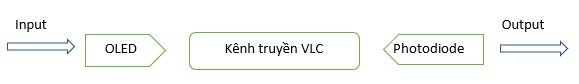
\includegraphics [scale=0.9] {Image/block_chart}
	\caption{Sơ đồ khối hệ thống quang không dây}
\end{figure}

\subsection{\ac{oled}}
\paragraph{\ac{oled} - Công nghệ của tương lai:}

Trong thập kỷ qua, chúng ta đã chứng kiến sự phát triển mạnh mẽ của công nghệ \ac{ssl}. Theo Allied Market Research \cite{ssl_market}, giá trị thị trường của \ac{ssl} năm 2019 là 32.65 tỷ USD và dự kiến đạt 74.25 tỷ USD vào năm 2027, phát triển dựa trên 3 công nghệ chính là \ac{led}, \ac{pled} và \ac{oled}. Theo Businesswire\cite{oled_market}, giữa thời kỳ khủng hoảng COVID-19, thị trường \ac{oled} dùng cho chiếu sáng vẫn đạt 67.1 triệu USD vào năm 2020 và có thể đạt được 291.1 triệu USD vào 2027, với tốc độ tăng trưởng hàng năm đạt 23.3 \% từ 2020 đến 2027. Tập trung trong các lĩnh vực như nhà ở, văn phòng, công nghiệp, bệnh viện, ngoài trời, cửa hàng và tự động hóa. Những lĩnh vực như kiến trúc, bệnh viện, cửa hàng sẽ là những lĩnh vực đi đầu. Kế đến, tự động hóa cũng nhận được sự cam kết phát triển triển của các công ty, ví dụ như BMW nếu như tuổi thọ và độ tin cậy được cải thiện. Cuối cùng, các lĩnh vực như nhà ở, văn phòng, ngoài trời sẽ đi theo sau nếu như giá sản xuất giảm và tuổi thọ được kéo dài.

\begin{figure} [ht]
	\centering
	\captionsetup{justification=centering}
	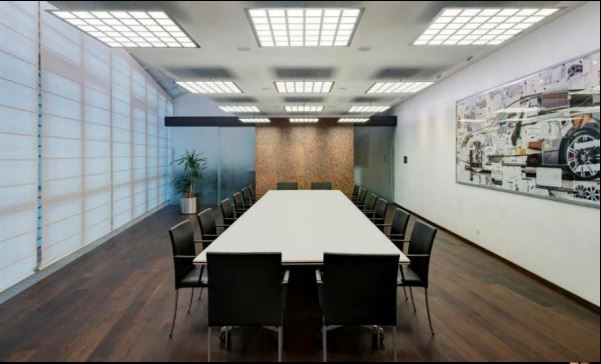
\includegraphics [scale=0.7] {Image/OLED_in_office}
	\caption{\ac{oled} được ứng dụng làm đèn chiếu sáng trong văn phòng \cite{oledworks}}
\end{figure}

\ac{oled} mang lại ánh sáng mềm mại, không đổ bóng, không chói mắt, mát khi chạm vào. Đó là thứ ánh sáng thuần khiết và mang một vẻ đẹp huyền diệu. Khi so sánh với \ac{led}, \ac{oled} mang những ưu điểm nổi trội như  màu sắc dễ chịu, khả năng kiểm soát màu sắc tốt, diện tích phát xạ lớn, ... Tuy nhiên, tuổi thọ, hiệu suất và đặc biệt là chi phí sản xuất cao vẫn là những khuyết điểm lớn của \ac{oled} khi so với \ac{led}.

\begin{figure} [ht]
	\centering
	\captionsetup{justification=centering}
	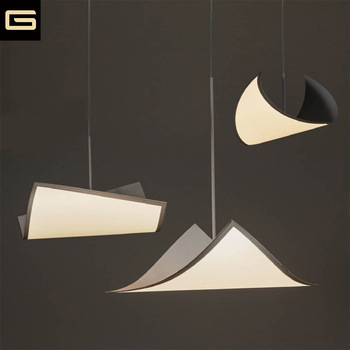
\includegraphics [scale=0.5] {Image/oled}
	\caption{Khả năng tùy chỉnh hình dạng của \ac{oled}}
\end{figure}

\paragraph{\ac{oled} trong hệ thống \ac{vlc}:}
Từ những ưu điểm và tiềm năng như trên \ac{oled} sẽ một công nghệ mạnh mẽ cho lĩnh vực chiếu sáng trong tương lai, nhưng giờ đây, ngoài khả năng chiếu sáng, khoảng băng tần khả kiến của chúng còn có thể sử dụng cho truyền nhận dữ liệu không dây, mà ở đó cũng chính là nguồn phát dữ liệu. 

Cả \ac{led} và \ac{oled} đều một lựa chọn rất được các nhà nghiên cứu quan tâm để dùng làm nguồn sáng cho công nghệ \ac{vlc}. Tuy nhiên, \ac{oled} lại có băng thông điều chế thấp hơn rất nhiều so với đèn \ac{led} thông thường. Không giống như \ac{led} thông thường, \ac{oled} là tập hợp các phân tử hữu cơ, do đó độ linh động của nó thấp hơn nhiều so với các thiết bị silicon khác, kết quả là sẽ giới hạn băng thông điều chế của nó. Băng thông điều chế của \ac{oled} còn phụ thuộc vào nhiều thứ, như là quá trình sản xuất, kích cỡ...nhưng băng thông thông thường của chúng chỉ dừng lại ở vài trăm KHz.

Trước đây, có rất ít nghiên cứu sử dụng \ac{oled} trong \ac{vlc}. Tiêu biểu như, tốc độ là 51.6 Mb/s với \ac{oled} 3 màu băng thông là 460 kHz, điều chế \ac{ofdm}, cân bằng MLP-ANN, với khoảng cách là 5 cm \cite{vlc-oled-51.6Mbps}; tốc độ 1.4 Mb/s đạt được với điều chế discrete multitone khi băng thông nhỏ hơn 100 kHz \cite{vlc-oled-1.4Mbps}; và tốc độ 2.7 Mb/s với \ac{oled} trắng và cân bằng thời gian thực ANN với băng thông là 93 kHz \cite{vlc-oled-2.7Mbps}; truyền thời gian thực tốc độ 138 kp/s, băng thông 7 kHz, điều chế DPPM, khoảng cách 40 cm \cite{vlc-oled-138kbps}.  
\begin{figure} [ht]
	\centering
	\captionsetup{justification=centering}
	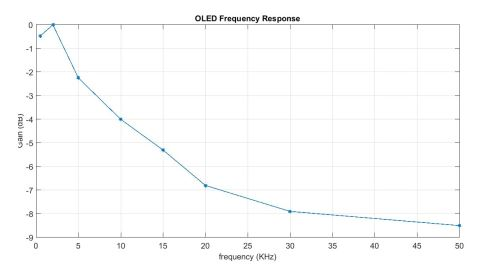
\includegraphics [scale=1] {Image/OLED_frequency_response}
	\caption{Đáp ứng của \ac{oled} Lumiable sáng trằng tiêu chuẩn}
\end{figure}
\subsection{Photodiode}
Photodiode là một diode bán dẫn thực hiện biến đổi photon thành dòng điện theo hiệu ứng quang điện, các photon có thể thuộc vùng phổ của ánh sáng khả kiến, hồng ngoại hay tử ngoại,... Photodiode sử dụng trong khảo sát là ADP do thorlab sản xuất, nó gồm một photodiode silic và một bộ khuyếch đại biến đổi trở kháng TIA (Transimpedance Amplifier). Bộ thu được thiết kế để thu được tín hiệu quang có bước sóng từ 400 đến 1000 nm, độ lợi có thể thay đổi từ 0 đến 70dB, điện áp ra 5V với trở kháng tải ngoài 50 Ω .
\begin{figure} [ht]
	\centering
	\captionsetup{justification=centering}
	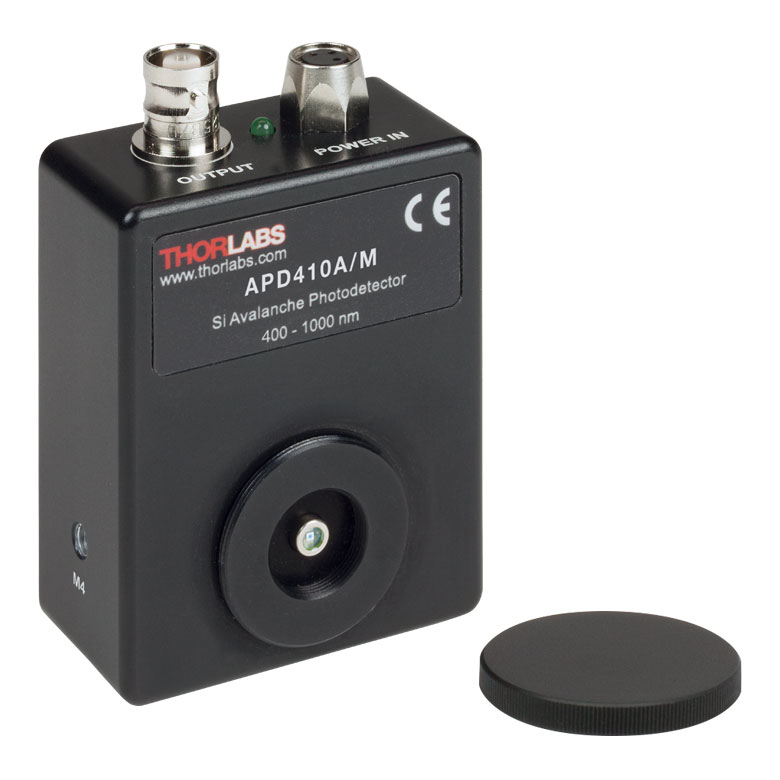
\includegraphics [scale=0.3] {Image/APD410A_M}
	\caption{Bộ thu quang APD410A/M của Thorlab}
\end{figure}
\subsection{Kênh truyền quang}
Kênh truyền quang học đã được chứng minh là một kênh truyền tuyến tính, biến đổi theo thời gian, không nhớ với đáp ứng xung là hữu hạn theo thời gian. Đặc điểm cơ bản của kênh truyền quan là phần suy hao quang học, việc mô hình hóa kênh truyền quang để thể hiện gồm 2 loại tia truyền: \ac{los} và \ac{nlos}.Việc truyền tốc độ cao sẽ khiến băng thông tín hiệu lớn, khi băng thông coherence lớn, kênh truyền quang được xem như là kênh truyền chọn lọc tần số. Trong đó loại tia truyền\ac{los} cung cấp khả năng cường độ tốt hơn tại bộ phát và thu và băng thông coherence tốt hơn, nó thích hợp với các đường truyền có tốc độ cao, tuy nhiên không phù hợp với các ứng dụng di động cao, đường truyền dễ bị bẻ gãy hoặc bị gián đoạn. Trong khi đó, truyền thông bằng \ac{nlos} cung cấp biên độ thấp hơn, băng thông coherence nhỏ hơn tuy nhiên độ di động cao hơn nhiều so với truyền thông \ac{los} do \ac{nlos} khai thác các đặc tính phản xạ của các đối tượng, cường độ bức xạ tại máy thu, đồng thời truyền thông \ac{nlos} có thể được tăng cường bằng cách khuếch tán. 
\begin{figure} [ht]
	\centering
	\captionsetup{justification=centering}
	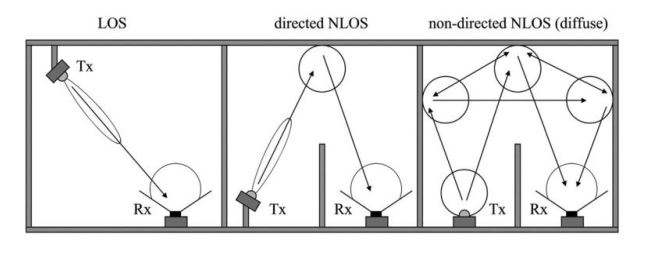
\includegraphics [scale=1] {Image/LOS_NLOS}
	\caption{Mô hình truyền thông \ac{los} và \ac{nlos}}
\end{figure}

Đáp ứng xung của kênh truyền có thể được mô hình hóa theo phương trình bên dưới cho cả truyền thông
LOS và NLOS:
\begin{equation}
h(t) = g_{h(opt)}U(t) \frac{6a^6}{(t+a)^7}
\end{equation}
Trong đó: g là độ lợi của kênh truyền, U(t) là hàm bước, a là băng thông trải trễ của kênh
truyền. Tuy nhiên trong truyền thông \ac{los}, do khoảng cách giữa máy phát và máy thu là ngắn (khoảng 1m). Ngoài ra, không giống như trong truyền thông vô tuyến, trong truyền thông \ac{los}, băng thông coherence được định nghĩa là tốc độ chênh lệch của từng bước sóng trong nguồn phát Laser hay \ac{led}. Khi đó, nếu khoảng cách máy phát và máy thu đủ xa thì ta mới thấy sự chênh lệch của các bước sóng nội tại của nguồn, lúc đó ta xem như có nhiều tia sáng trong một luồng \ac{los}, nhiễu \ac{isi} sẽ xuất hiện, trong trường hợp nhiễu \ac{isi} sẽ xuất hiên, khoảng guard interval sẽ được thêm vào để giảm lượng chồng lấn giữa các xung, qua đó làm giảm hiệu suất sử dụng phổ. Tổng quát, trong truyền thông \ac{los}, ta xem như đáp ứng xung của kênh truyền là: $h(t) = \delta (t)$

\subsection{Mạch pre-emphasis: \cite{pre-emphasis}}

Để vượt qua giới hạn băng thông điều chế hẹp của nguồn sáng, mạch pre-emphasis đã được sử dụng để tăng băng thông cho hệ thống \ac{vlc} dùng \ac{oled}. 

Về cơ bản, mạch pre-emphasis điều chỉnh lại bộ lọc band-pass tích cực bằng cách sử dụng OP-AMP với mục đích là bù lại phần tần số từ DC đến 100kHz. Băng thông điều chế trong hệ thống \ac{oled} \ac{vlc} có thể tăng 45 lần.
 
\section{Ứng dụng neural networks để phân loại tín hiệu}
\subsection{Giới thiệu}
Nguyên lý và thiết kế của mạng neural nhân tạo đã có sự phát triển vượt bật trong 20 năm gần đây. Có nhiều ứng dụng ảnh hưởng trực tiếp đến việc xử lý số tín hiệu. Neural network có thể học được trong môi trường giám sát và không giám sát trở nên rất phù hợp trong việc giải quyết những khó khăn của trong vấn đề xử lý tín hiệu. \cite{NN-DSP}

Một trong những xu hướng chính trong việc ứng dụng neural networks vào xử lý số tín hiệu là phân loại tín hiệu. Tín hiệu được phân loại có thể là tín hiệu thu được từ cảm biến \cite{8940077}, tín hiệu điện não đồ \cite{eeg}, tín hiệu điện tim đồ \cite{ecg}, ...Trong báo cáo này, chúng tôi sẽ ứng dụng các phương pháp phân loại tín hiệu bằng neural networks cho tín hiệu thu được từ hệ thống \ac{vlc}.

Tín hiệu ban đầu sau khi đi qua một loạt khối và kênh truyền đã bị nhiễu, méo dạng, không còn giống như tín hiệu ban đầu. Việc sử dụng neural network sẽ giúp phân biệt được các mức ngõ ra của tín hiệu. Mô hình được sử dụng ở đây thuộc loại là phân loại (classification). Với ngõ vào của mô hình là tín hiệu ngõ ra bị nhiễu thu được tại photodiode, ngõ ra của mô hình là mức tín hiệu đúng.

Trước đây, đã có khá nhiều nghiên cứu trên lĩnh vực trên như: Dùng \ac{cnn} để giải điều chế BPSK \cite{cnn-bpsk}, sử dụng Deep Belief Network để giải điều chế với kênh truyền AWGN \cite{dcnn}, ...Báo cáo khoa học \cite{demod-with-ML} thực hiện đề tài tương tự đối với hệ thống \ac{vlc} dùng \ac{led}.

Báo cáo này sẽ phát triển ý tưởng trên thông qua việc sử dụng 3 phương pháp: \ac{pnn}, \ac{grnn}, \ac{dtnn} trên hệ thống \ac{vlc} dùng \ac{oled}.
\subsection{Probabilistic Neural Networks}
Neural network đã thường xuyên được ứng dụng trong việc phân loại mẫu bằng cách học từ những ví dụ. Những phương pháp hiện tại như backpropagation yêu cầu một thời gian tính toán dài dành cho việc training và dễ bị mắc phải việc tìm sai cực tiểu. Để khắc phục được vấn đề này, một phương pháp phân loại dựa trên những định lý thống kê đã có được tìm ra. 

\ac{pnn} là một bộ phân loại Bayes-Parzen, nền tảng của phương pháp này xuất hiện từ thập niên 1960, tuy nhiên phương pháp này không phổ biến vì năng lực tính toán yếu của máy tính lúc bấy giờ. \ac{pnn} được giới thiệu đầu tiên bởi Specht (1990). Ông đã chỉ ra cách mà bộ phân loại Bayes-Parzen có thể được chia thành một số lượng lớn các quy trình đơn giản được thực hiện trong mạng neurons nhiều lớp, mỗi quy trình có thể chạy song song độc lập.
\paragraph{Bộ phân loại Bayes:} \cite{ml_coban}
Xét một bài toán với $K$ lớp $(1, 2, …, k, ..., K)$. Giả sử có một điểm dữ liệu $x \in \mathbb{R}^d$, xác suất để điểm dữ liệu này rơi vào class $k$.
\begin{equation}
p(y=k \vert x)
\end{equation}
Hoặc viết gọn thành $p(k|x)$.
Tức tính xác suất để đầu ra là class $k$ biết rằng đầu vào là vector $x$.
Từ đó có thể giúp xác định được class của điểm dữ liệu đó bằng cách chọn ra class có xác suất cao nhất: 
\begin{equation}
k = \arg \underset{k \in {{1, ..., k}}} {\mathrm{max}} p(k|x)
\end{equation}
Biểu thức trên khó có thể tính trực tiếp, thay vào đó quy tắc Bayes thường được sử dụng:
\begin{equation}
  k =  \arg\max_k p(k | \mathbf{x}) \ 
     =  \arg\max_k \frac{p(\mathbf{x} | k) p(k)}{p(\mathbf{x})} \ 
       =  \arg\max_k p(\mathbf{x} | k) p(k) \ 
\end{equation}
Trong đó $p(k)$ có thể được hiểu là xác suất để một điểm rơi vào lớp k. Giá trị này có thể được tính bằng Maximum likehood estimation, tức tỉ lệ số điểm dữ liệu trong tập training rơi vào class này chia cho tổng số lượng dữ liệu trong tập training, hoặc cũng có thể ước lượng bằng MAP estimation. Phần còn lại $p(x|k)$ là phân phối của các điểm dữ liệu trong lớp k (\ac{pdf}) 

Vấn đề lớn nhất với phương pháp phân loại Bayes là \ac{pdf} thường chưa biết. Thông thường thì phân phối được giả sử là Gaussian. Độ chính xác của đường biên phụ thuộc nhiều vào độ chính xác của việc ước lượng \ac{pdf}. Các phương pháp ước lượng thông dụng có thể kể đến như: Parzen windows, k nearest neighbor, Potential function. \cite{PNN_chapter}
\paragraph{Ước lượng Parzen (Parzen window):} \cite{Implementing-PNN}
Đây là phương pháp phổ biến nhất được Parzen (1962) chỉ ra để có thể ước lượng được $f(X)$.
\begin{equation}
f(x) \approx f_n(X) = \frac{1}{n\lambda} \sum_{i=1}^n g(\frac{X - X_{Ai}}{\lambda})
\end{equation}
Trong đó: $g$ gọi là window hoặc hàm kernel, $X$ là biến ngẫu nhiên của một điểm trong không gian mẫu, $X_{Ai}$ là biến ngẫu nhiên độc lập có phân phối giống như X,  $\lambda$ là chiều rộng của window, tham số độ mượt, hay đơn giản là kích thước kernel,  là hàm của n sao cho:
\begin{equation}
\lim_{n\to\infty} \lambda = 0 \hspace{0.5 cm} and  \hspace{0.5 cm} \lim_{n\to\infty} n\lambda = \infty
\end{equation}
Cacoullos (1966) đã mở rộng kết quả của Parzen để giải quyết trường hợp đa biến. Trong trường hợp cụ thể là Gaussian kernel, ước lượng đa biến có thể được biểu diễn như sau: \cite{PNN-original}
\begin{equation}
f_A(X) = \frac {1}{(2\pi)^{p/2}\sigma^p} \frac{1}{m} \sum ^m _{i=1} \times \exp (-\frac{(X-X_{Ai})^T(X-X_{Ai})}{2\sigma^2})
\label{eqn:cacoullos}
\end{equation}
 Trong đó:
 \begin{itemize}
	 \item $i$ là số mẫu
	 \item $m$ là tổng số mẫu training
	 \item $X_{Ai}$ là mẫu training thứ i của loại $\theta_A$
	 \item $\sigma$ là độ lệch chuẩn
	 \item $p$ là chiều của không gian đo lường
 \end{itemize}
\paragraph{Kiến trúc} Mạng PNN được Specht (1990) giới thiệu gồm có 4 layers: \cite{PNN-original} \cite{PNN_chapter}
\begin{enumerate}
	\item Input layer: là tập hợp $p$ các kết nối để lấy vector ngõ vào và truyền chúng cho các layer tiếp theo.
	\item Pattern layer: quá trình này sẽ được thực hiện thông qua 2 bước:
	
	Bước thứ nhất: mỗi unit sẽ so sánh mẫu dành riêng của nó với vector ngõ vào bằng cách tính khoảng cách $D(x, X_i^{(j)})$. Giá trị của $D(x, X_i^{(j)})$ thể hiện mức độ đóng góp của mẫu training cho ngõ ra trong mẫu test. Nếu $D(x, X_i^{(j)})$ nhỏ, có nghĩa là nó có nhiều đóng góp cho ngõ ra. Nếu $D(x, X_i^{(j)})$ lớn, có nghĩa là nó có rất ít đóng góp cho ngõ ra. Nếu $D(x, X_i^{(j)})$ bằng 0, có nghĩa là dữ liệu test giống với dữ liệu train và ngõ ra của dữ liệu test sẽ là ngõ ra của mẫu train. 
	\begin{itemize}
		\item Thực hiện phép tính dot product: (Specht, 1990)
		\begin{equation}
		D(x, X_i^{(j)}) = \sum^p_{k=1}x_k \cdot X_{i,k}^{(j)}
		\end{equation}
		Trong đó: $x_k$ là phần tử thứ $k$ của vector ngõ vào, $X_{i,k}$ là phần tử training thứ $k$ của mẫu thứ $i$ thuộc về lớp j. Cả 2 vectors phải được chuẩn hóa trước khi thực hiện phép nhân.
		\item Khoảng cách Euclidean:
		\begin{equation}
		D(x, X_i^{(j)}) = \sqrt{\sum ^p_{i=1}(x_i - X_i^{(j)})^2}
		\end{equation}
		\item Khoảng cách Manhattan (or city block):
		\begin{equation}
		D(x, X_i^{(j)}) = \sum ^p_{i=1}|x_i - X_i^{(j)}|
		\end{equation}
	\end{itemize}
	Bước thứ hai: Thay vì sử dụng hàm sigmoid thông dụng trong backprobagation, hàm không tuyến tính (kernel) được sử dụng. Một số hàm dành cho những khoảng cách ở trên như:
	\begin{itemize}
		\item Cho dot product: (Specht, 1990)
		\begin{equation}
		K(x, X_i^{(j)}) = \exp{(\frac{D(x, X_i^{(j)})-1}{2\sigma^2})}
		\end{equation}
		\item Cho khoảng cách Euclidean:
		\begin{equation}
		K(x, X_i^{(j)}) = \exp{(\frac{-D(x, X_i^{(j)})}{2\sigma^2})}
		\end{equation}
		\item Cho khoảng cách Manhattan:
		\begin{equation}
		K(x, X_i^{(j)}) = \exp{(\frac{-D(x, X_i^{(j)})^2}{2\sigma^2})}
		\end{equation}
	\end{itemize}
	Từ đó có thể ước lượng hàm \ac{pdf} bằng công thức:
	\begin{equation}
	\hat f_{j, n} = \frac{1}{\lambda _{nj}^p}\sum_{i=1}^{n_j}K(x, X_i^{(j)})
	\end{equation}
	\item Summation layer: các units đơn giản là tính tổng của các neuron ở pattern layer tương ứng với loại mà mẫu training được chọn. Một đặc trưng khác có thể kết hợp trong summation layer là tính hệ số: $\hat d_j(x) = p(x 		k)p(k)$ để dùng bộ phân loại Bayes.
	\item Output layer (Decision layer): có vai trò là chọn $\hat d_j(x)$ lớn nhất và khai báo vector đầu vào x thuộc lớp j
\end{enumerate}
\begin{figure} [ht]
	\centering
	\captionsetup{justification=centering}
	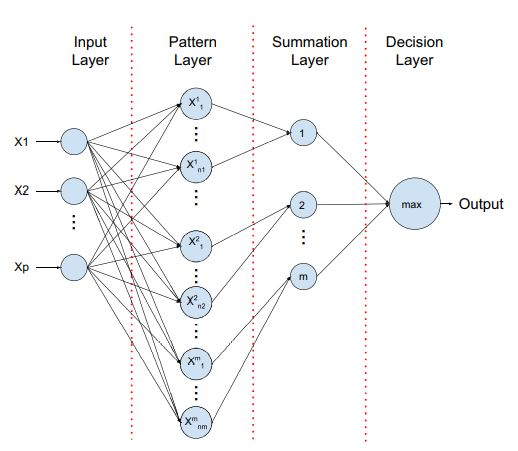
\includegraphics [scale=1] {Image/PNN_architecture}
	\caption{Kiến trúc của \ac{pnn}}
\end{figure}
\paragraph{Ưu điểm:}
\begin{itemize}
	\item Ưu điểm lớn nhất của \ac{pnn} là có thể training dễ dàng và nhanh chóng
	\item Có thể ứng dụng cho hệ thống real time
	\item Mẫu thêm vào có thể được giám sát và lưu trữ trong mạng
	\item Sự tổng quát hóa được cải thiện và đường biên đươc quyết định trở nên phức tạp hơn.
\end{itemize}
\paragraph{Nhược điểm:}
\begin{itemize}
	\item Chậm hơn multilayer perceptron về khía cạnh phân loại dự liệu mới
	\item Yêu cầu nhiều không gian bộ nhớ để lưu trữ mô hình.
\end{itemize}
\paragraph{Những ứng dụng của \ac{pnn}} \cite{PNN_chapter}
\begin{itemize}
	\item Phân loại những mẫu dữ liệu có nhãn 
	\item Phân loại những mẫu có dữ liệu là hàm mật độ xác suất thay đổi theo thời gian
	\item Xử lý số tín hiệu, với dạng sóng là mẫu dữ liệu
	\item Thuật toán không giám sát với dữ liệu chưa dán nhãn
\end{itemize}
\subsection{General Regression Neural Networks}
\ac{grnn} là một loại single-pass neural networks, được đề xuất bởi Donald J. Specht (1991). Dựa trên nền tảng toán học \ac{grnn} cung cấp một mạng có thể dể dàng sử dụng mà có thể giảm thời gian training và tăng hiệu năng cho mô hình.
\paragraph{General regression:} Giả sử $f(x, y)$ biểu diễn cho một hàm mật độ xác suất kết hợp liên tục của vector biến ngẫu nhiên x và biến vô hướng y (scalar). Gọi X là giá trị cụ thể của biến ngẫu nhiên x, trung bình có điều kiện của y được cho bởi X (còn được gọi là hồi quy của y trên X) là:
\begin{equation}
\label{eqn:grnn-1}
E[y|X] = \frac{\int _{-\infty}^{\infty}yf(X, y)dy}{\int _{-\infty}^{\infty}f(X, y)dy}.
\end{equation}
Khi hàm mật độ $f(x, y)$ là chưa biết, nó thường được ước lượng bằng mẫu giám sát x và y. Để ước lượng phi tham số cho $f(x, y)$, chúng ta có thể sử dụng phương pháp ước lượng đồng nhất được cho bởi Parzen và ứng dụng cho trường hợp đa biến của Cacoullos. Xác suất ước lượng $\hat f(X, Y)$ phụ thuộc vào giá trị $X^i$ và $Y^i$ của biến ngẫu nhiên x và y, khi n là số lượng mẫu giám sát và p là số chiều của vector biến x.
\begin{equation}
\label{eqn:grnn-2}
\hat f(X, Y) = \frac{1}{(2\pi)^{(p+1)/2}\sigma^{p+1}}.\frac{1}{n}\sum^n_{i=1}\exp[-\frac{{(X-X^i)}^T(X-X^i)}{2\sigma^2}].\exp[-\frac{{(Y-Y^i)}^2}{2\sigma^2}].
\end{equation}
Thay \ref{eqn:grnn-1} vào \ref{eqn:grnn-2}, chúng ta được:
\begin{equation}
\label {eqn:grnn-3}
\hat Y(X) = \frac{\sum_{i=1}^n\exp[-\frac{{(X-X^i)}^T(X-X^i)}{2\sigma^2}]\int _{-\infty}^{\infty}y\exp[-\frac{{(y-Y^i)}^2}{2\sigma^2}]dy}{\sum_{i=1}^n\exp[-\frac{{(X-X^i)}^T(X-X^i)}{2\sigma^2}]\int _{-\infty}^{\infty}\exp[-\frac{{(y-Y^i)}^2}{2\sigma^2}]dy}
\end{equation}
Trong đó: $D^2_i = {(X-X^i)}^T(X-X^i)$ là khoảng cách Euclidien. Từ đó, chúng ta có hàm activation là $\exp(-D^2_i/2\sigma^2)$. 

Chúng ta chỉ có một tham số chưa biết là $\sigma$. Quá trình training sẽ tìm ra điểm tối ưu của $\sigma$ bằng cách tìm giá trị nhỏ nhất của \ac{mse} \cite{grnn_github}
\paragraph{Kiến trúc:}\ac{grnn} có 4 layers, với 2 layers đầu tiên tương tự như \ac{pnn}:
\begin{enumerate}
	\item Input layer: có nhiệm vụ chuyển giá trị ngõ vào sang các layer tiếp theo.
	\item Pattern layer: tính toán khoảng cách và hàm activation.
	\item Summation layer: dựa trên biểu thức \ref{eqn:grnn-3}, chúng ta chia thành 2 neurons là Numerator (tử số) neuron và Denominator (mẫu số) neurons. Numerator neuron tính tổng các giá trị trọng số từ pattern layer, Denominator neuron tính tổng của các phép nhân giữa trọng số của pattern layer và giá trị đích thực tế.
	\item Output layer: chia giá trị thu được từ Numerator neuron cho giá trị của Denominator và sử dụng kết quả đó để dự đoán giá trị đích.
\end{enumerate}
\begin{figure} [ht]
	\centering
	\captionsetup{justification=centering}
	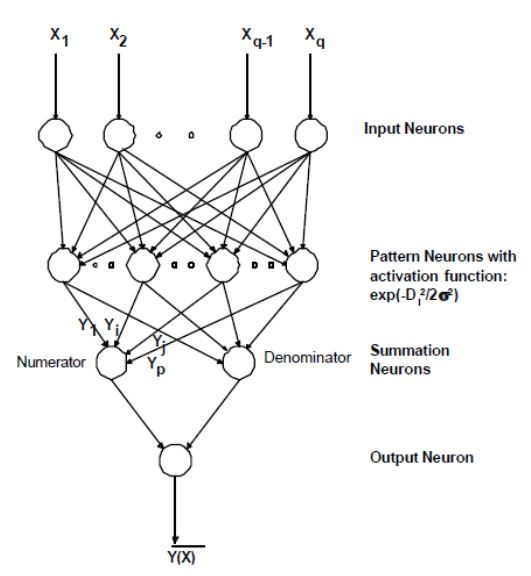
\includegraphics [scale=0.8] {Image/GRNN_model}
	\caption{Kiến trúc của \ac{grnn}}
\end{figure}
\paragraph{Ưu điểm:}
\begin{itemize}
	\item Quá trình học single-pass, không yêu cầu backpropagation
	\item Độ chính xác xao dành cho việc ước lượng
	\item Có thể xử lý được nhiễu ở ngõ vào 
	\item Chỉ yêu cầu một lượng nhỏ dữ liệu
\end{itemize}
\paragraph{Nhược điểm:}
\begin{itemize}
	\item Kích thước của nó có thể rất lớn, làm tăng chi phí tính toán
	\item Không có phương pháp tối ưu nào để cải thiện nó
\end{itemize}

\subsection{Deep Tensor Neural Networks \cite{Yu2012LargeVS}}
\paragraph{Giới thiệu}
\ac{dtnn} là một mô hình được mở rộng từ \ac{dnn}. Ý tưởng cơ bản của \ac{dtnn} đến từ việc, những nhận biết của chúng ta đến từ nhiều yếu tố tương tác với nhau và dự đoán ngõ ra. Để thể hiện sự tương tác, chúng ta chiếu ngõ vào thành hai vùng không gian con tuyến tính.
\paragraph{Kiến trúc}
\begin{figure} [ht]
\centering
\captionsetup{justification=centering}
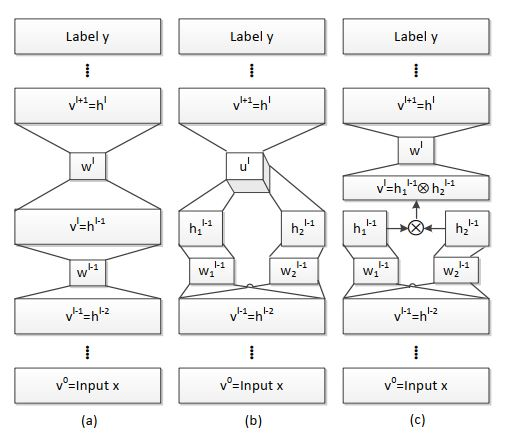
\includegraphics [scale=1] {Image/DTNN}
\caption{Kiến trúc của \ac{dnn} và \ac{dtnn}. (a) DNN. (b) DTNN: hidden layer $h^{l-1}$ bao gồm 2 phần $h_1^{l-1}$ và $h_2^{l-1}$. Hidden layer $h^l$ là tensor layer kết nối weight $u^l$ với three way tensor. (c) Cách biểu diễn khác của (b): tensor $u^l$ được thay thế bằng ma trận $w^l$ với $v^l$ được định nghĩa là tích vô hướng $h_1^{l-1} \otimes h_1^{l-1}$}
\end{figure}

Trong đó, ngõ vào của \ac{dtnn} là $x$, $I \times 1$ vector, và ngõ ra là $y$, $C \times 1$ vector.
Hidden layer $h^{l-1}$ được chia thành 2 phần $h_1^{l-1}$ ($K_1^{l-1} \times 1$ vector) và  $h_2^{l-1}$ ($K_2^{l-1} \times 1$ vector).Hai phần này được kết nối với nhau bởi hidden layer $h^l$ thông qua một three way tensor $u^l$ được biểu diễn bằng hình lập phương như torng hình.

Trong hình (c), góc nhìn thay thế của \ac{dtnn} được định nghĩa bởi:
\begin{equation}
v^l = vec (h_1^{l-1}(h_2^{l-1})^T)
\end{equation}
Cách viết lại này cho phép chúng ta kết nối giữa những layer thông thường và tensor layers. Khi đó hidden layer $h^l$ có thể được xem như là layer thông thường và có thể được học bằng thuật toán backpropagation. Tuy nhiên với hidden layer $h^{l-1}$ vẫn chứa 2 thành phần $h_1^{l-1}$ và $h_2^{l-1}$, chúng được xác định bời 2 ma trận weights $w_1^{l-1}$ và $w_2^{l-1}$. Chúng ta gọi nó là double-projection layer. 

Tóm lại có 3 loại layers trong \ac{dtnn}: hidden layer thông thường, double-projection layer và softmax layer (sigmoid layer với bài toán binary classification) kết nối layer cuối cùng với nhãn. Với layer dầu tiên, ta có:
\begin{equation}
v^l = v^0 = x
\end{equation}
Với layers $l > 0$, nếu layer phía trước là hidden layer thông thường $v^l = h^{l-1}$. Với hidden layer thông thường ta có:
\begin{equation}
h_i^l = f(z^l(v^l)) = f((w^l)^Tv^l + a^l), 
\end{equation}
Trong đó, $w^l$ là ma trận trọng số, $a^l$ là bias, $f(x)$ là hàm activation.
Với Double-projection layer:
\begin{equation}
h_i^l = f(z_i^l(v^l)) = f((w_i^l)^Tv^l + a-i^l)
\end{equation}
Trong đó $i = {1, 2}$ là số thứ tự các phần.
\section{Ứng dụng neural networks để giảm méo dạng phi tuyến}
\subsection{Giới thiệu}

Ước lượng được tín hiệu sạch từ tín hiệu bị nhiễu, méo dạng, ... là một vấn đề rất quan trọng trong việc xử lý số tín hiệu. Trong những năm gần đây, với sự phát triển nhanh chóng của neural networks, nó ngày càng trở nên mạnh mẽ và những ứng dụng của nó cũng phổ biến hơn. Ngoài việc dùng để phân loại tín hiệu như đã trình bày ở chương trước, nó còn thể được ứng dụng vào việc hiệu chỉnh lại tín hiệu bị nhiễu hay méo dạng.

Trước đây, có khá ít nghiên cứu trong lĩnh vực này, tiêu biểu là: sử dụng Adversarial autoencoder để làm giảm méo dạng phi tuyến \cite{segan}, tăng cường giọng nói bằng \ac{dae} \cite{se_dae}, ...

\subsection{Autoencoder Neural Networks}
Autoencoder được giới thiệu đầu tiên năm vào thập niên 1980 bởi Hinton và nhóm PDF (Rumelhart và những người khác, 1986) để giải quyết vấn đề về backpropagation khi dữ liệu không có được dán nhãn. \ac{ae} là một loại neural networks thuộc loại unsupervised learning, mục tiêu là học đặc tính của dữ liệu. 
\begin{figure} [ht]
\centering
\captionsetup{justification=centering}
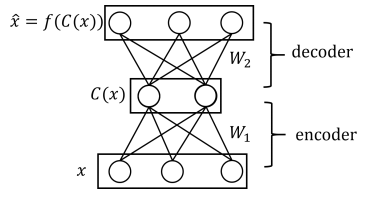
\includegraphics [scale=1] {Image/autoencoder_simple_model}
\caption{Kiến trúc đơn giản của Autoencoder}
\end{figure}
Xét một mô hình Autoencoder đơn giản,\cite{autoencoder_lecture_SNU} với 3 layers. Trong đó, layer ngõ vào và layer ngõ ra có số neuron bằng nhau, hidden layer thường có số neuron ít hơn. Ma trận $W_1$ là trọng số kết nối layer ngõ vào và hidden layer, $W_2$ là kết nối hidden layer và layer ngõ ra. Thông thường, $W_2 = W_1^T$, chúng ta đặt $W_1 = W$ và $W_2 = W^T$. Ngõ vào $x$ khi đi qua layer ngõ vào sẽ tạo thành: $h = \sigma(Wx + b)$ ở hidden layer và  $\hat x = \sigma(W^Th+c)$ ở ngõ ra. 

Mục tiêu cơ bản của autoencoder là tạo ra ngõ ra $\hat x$ càng gần với ngõ vào $x$ càng tốt. Tuy nhiên, nó không thể luôn được thực hiện nếu số neuron ở hidden layer nhỏ hơn nhiều so với ở layer ngõ vào và ngõ ra. Trong trường hợp đó, giá trị $h$ ở ngõ vào cần được nén lại như dữ liệu tại ngõ vào. Vì vậy, chúng ta có thể viết:
\begin{equation}
h = C(x).
\end{equation}
Khi đó, neural network gồm layer ngõ vào và hidden layer gọi là encoder, gồm hidden layer và layer ngõ ra gọi là decoder, chúng ta viết:
\begin{equation}
\hat x = f(C(x)).
\end{equation}
Để có thể thấy được cách mà encoder-decoder hoạt động, gọi tập dữ liệu là $D = {{x^{(i)}}_{i=1}^T}$, chúng ta viết:
\begin{equation}
\hat x^{(i)} = f(C{x^{(i)}}).
\end{equation}
Hàm lỗi thường được cho bởi $L^2$ error:
\begin{equation}
E = \frac {1}{2} \sum _i |\hat x ^ {(i)} - x^{(i)}|^2 = \frac{1}{2} \sum _i \sum _k |\hat x_k ^ {(i)} - x_k^{(i)}|, 
\end{equation}
Sau đó, chúng ta có thể dùng backpropagation để training như thông thường.
\paragraph{Những mô hình Autoencoder} về cơ bản có 7 loại như sau: \cite{autoencoder_type}
\begin{itemize}
	\item Denoising Autoencoder
	\item Sparse Autoencoder
	\item Deep Autoencoder
	\item Contractive Autoencoder
	\item Undercomplete Autoencoder
	\item Concolutional Autoencoder
	\item Variational Autoencoder
\end{itemize}
\paragraph{Ứng dụng:} \cite{Autoencoder_apps}
\begin{itemize}
	\item Giảm số chiều dữ liệu 
	\item Phục hồi thông tin
	\item Phát hiện tương đồng
	\item Xử lý ảnh: tái tạo hình ảnh, tô màu hình ảnh, tạo ra ảnh với độ phân giải cao, ...
	\item Thay đổi đặc trưng và giảm nhiễu
\end{itemize}
\subsection{Denoising Autoencoder}
\ac{dae} được giới thiệu bởi Vincent (2008, 2010) và Glorot (2011), cung cấp một mạng cho phép tái tạo lại dữ liệu từ những điểm dữ liệu bị hư hại, nhiễu chính là loại hư hại được tác giả chọn để mô hình hóa. 

Chúng ta có $x \in \mathbb{R}^d$ là ngõ vào của mạng. $y \in \mathbb{R}^{d'}$ là ngõ ra của mạng, có thể được tính toán đơn giản như sau: $f_{\theta} (x) = s (Wx + b)$, trong đó ma trận $W \in \mathbb{R}^{d' \times d}$ và vector $b \in \mathbb{R}^{d'}$ là tham số của mạng, $s$ là hàm activation, thông thường là $sigmoid$. Chúng ta có thể viết, $\theta  = (W, b)$, hàm f được gọi là $encoder$.

Phía $decoder$ cũng tương tự như $encoder$, $g_{\theta'} (y) = t(W'y + b')$, trong đó $W \in \mathbb{R}^{d' \times d}$ và $b \in \mathbb{R}^d$. $t$ là hàm activation thông thường thì nên khác với $s$. Thông thường $W$ và $W'$ bị ràng buộc bởi $W' = W^T$, vấn đề này được điều chỉnh lại trong định lý của Vincent (2011).

Trong suốt quá trình training, mục tiêu của chúng ta là học tham số encoder $W$ và $b$, thêm vào đó chúng ta sẽ cần phải học tham số decoder $b'$. Chúng ta có thể làm được việc này bằng cách định nghĩa phân bố xác suất $p(\bar{x}|x, v)$, phần hư hại được điều khiển bởi $a$ tham số $v$. Chúng ta train trọng số autoencoder để có thể tái tạo lại $a$ tín hiệu đầu váo ngẫu nhiên từ phân bố của x có được từ phiên bản hư hại của nó $\bar{x}$, bằng cách chạy $encoder$ và $decoder$ tuần tự. Quá trình này có thể được mô tả bằng hàm mục tiêu:
\begin{equation}
\theta^*, \theta'^* = \underset{\theta, \theta'}{arg min} \mathbb{E}_{(X, \bar{X})}[L(X, g_{\theta'}(f_{\theta}(\bar{X}))]
\end{equation}
Trong đó $L$ là loss function như là squared error. Thông thường, chúng ta tối ưu hóa hàm mục tiêu bằng Stochastic Gradient Descent với mini-batches.  

Có khá nhiều tham số tinh chỉnh ở đây như phân bố xác suất, chuyển đổi hàm $s$ và $t$ và loss function. Đối với loss function, cho trường hợp $x$ liên tục, squared error có thể được sử dụng. Trong trường hợp $x$ là nhị phân hoặc $x \in  [0, 1]$, loss function thường được sử dụng là loss entropy:
\begin{equation}
L(x, z) = -\sum_{i=1}^D (x_i \log z_i + (1-x_i) \log (1-z_i)).
\end{equation}

Đối với hàm activation, lựa chọn thông thường là sigmoid $s(v) = \frac{1}{1+e^{-v}}$ cho cả encoder và decoder hoặc có thể sử dụng rectifier $s(v) = max(0, v)$ cho phần kết nối giữa encoder và decoder.

Một trong những tham số quan trọng nhất cảu denoising autoencoder là phân bố xác suất $p$. Với tín hiệu x liên tục, nhiễu Gausisan $p(\bar{x}|x, v) = N (\bar{x}|x, v)$ có thể được sử dụng. Đối với $x$ là nhị phân hoặc $x \in  [0, 1]$, nhiễu thường được sử dụng là masking noise, với mỗi $i \in 1, 2, ... d$, chúng ta lấy mẫu $\bar{x_i}$ độc lập.
\begin{equation}
p(\bar{x_i}|x_i, v) =     
	\begin{cases}
      0 & \text{with probability $\nu$}\\
      x_i & \text{otherwise.}\\
    \end{cases} 
\end{equation}

Trong đó $\nu$ là mức nhiễu. 

\section{Biến đổi Wavelet liên tục}
\subsection{Giới thiệu}
Trong xử lý tín hiệu, phép biến đổi Fourier là một công cụ quan trọng vì nó là cầu nối cho việc biểu diễn tín hiệu giữa miền không gian và miền tần số. Việc biểu diễn tín hiệu trong miền tấn số đôi khi có lợi hơn trong miền không gian. Tuy nhiên, biến đổi Fourier chỉ có thể cung cấp thông tin có tính toàn cục và chỉ thích hợp cho những tín hiệu tuần hoàn, không chứa các đột biến hoặc các thay đổi không dự báo được. Để khác phục được đặc điểm này, Gabor đã đã áp dụng phép biển đổi Short Time Fourier cho từng đoạn nhỏ của tín hiệu. Phép biển đổi này cho thấy mối liên hệ giữa không gian và tần số nhưng lại bị khống chế bởi nguyên lý bật định Heisenberg cho các thành phần tần số cao và thấp trong tín hiệu. Phép biến đổi wavelet và bước tiếp theo để khắc phục hạn chế này.

Năm 1975, Morlet, J., phát triển phương pháp đa phân giải. Trong đó, ông ta sử dụng một xung dao động, được hiểu là một “wavelet” cho thay đổi kích thước và so sánh với tín hiệu ở từng đoạn riêng biệt.  Kỹ thuật này bắt đầu với sóng nhỏ (wavelet) chứa các dao  động tần số khá thấp, sóng nhỏ này được so sánh với tín hiệu phân tích để có một  bức tranh toàn cục của tín hiệu ở độ phân giải thô. Sau đó sóng nhỏ được nén lại để nâng cao dần tần số dao động. Quá trình này gọi là làm thay đổi tỉ lệ phân tích; khi thực hiện tiếp bước so sánh, tín hiệu sẽ được nghiên cứu chi tiết ở các độ phân giải cao hơn, giúp phát hiện các thành phần biến thiên nhanh còn ẩn bên trong 
tín hiệu. 

Đối với hệ thống \ac{vlc} dùng \ac{oled}, vì sử dụng mạch pre-emphasis để tăng băng thông cho hệ thống nên tín hiệu thu được là phi tuyến
\subsection{Biến đổi wavelet thuận}
Gọi $f(x)$ là tín hiệu 1D, biến đổi wavelet liên tục của tín hiệu $f(x)$ sử dụng hàm wavelet $\Psi_0$ được biểu diễn bởi:
\begin{equation}
W(s, b) = \frac{1}{\sqrt{s}} \sum_{-\infty}^{+\infty} f(x)\Psi_0^*(\frac{x-b}{s})dx
\end{equation}
Trong đó:
\begin{itemize}
	\item $W(s, b)$ là hệ số biến đổi wavelet liên tục của $f(x)$
	\item $s$ là tỷ lệ (nghịch đảo của tần số)
	\item $b$ là dịch chuyển đặc trưng của vị trí
	\item $\Psi_0^*(x)$ là hàm liên hiệp phức của của wavelet $\Psi_0(x)$.
\end{itemize}

Phép biến đổi wavelet có độ linh động cao so với biến đổi Fourier vì không nhất thiết phải dùng một hàm wavelet cố định, mà có thể lựa chọn hàm wavelet khác nhau cho bài toán thích hợp. 

\begin{figure} [ht]
	\begin{subfigure}{0.3\textwidth}
		\centering
		\captionsetup{justification=centering}
		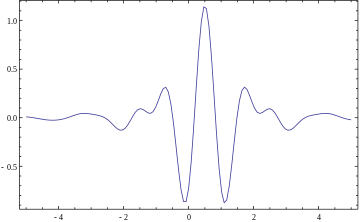
\includegraphics [width=\textwidth] {Image/meyer}
		\caption{Meyer}
	\end{subfigure}
	\hfill
	\begin{subfigure}{0.3\textwidth}
		\centering
		\captionsetup{justification=centering}
		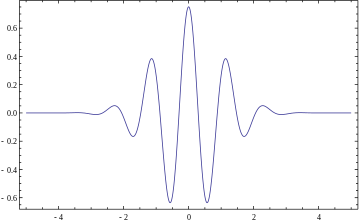
\includegraphics [width=\textwidth] {Image/morlet}
		\caption{Morlet}
	\end{subfigure}
	\hfill
	\begin{subfigure}{0.3\textwidth}
		\centering
		\captionsetup{justification=centering}
		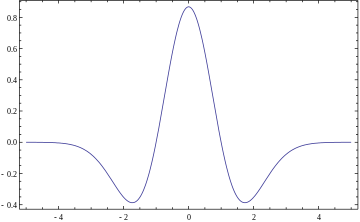
\includegraphics [width=\textwidth] {Image/mexh}
		\caption{Mexican hat}
	\end{subfigure}
\caption{Một số mother wavelet thông dụng cho \ac{cwt}}
\end{figure}

\paragraph{Độ rộng}
Quan hệ giữa độ rộng của hàm wavelet trong miền không gian và độ rộng trong miền tần số cho bởi nguyên lý bất định Heisenber. Nếu hàm wavelet bị hẹp về độ rộng trong miền không gian thì ngược lại, độ rộng của phổ tần số sẽ tăng lên. Vậy độ phân giải tối ưu trong miền tần số sẽ tương ứng với độ phân giải rất hạn chế trong miền không gian và ngược lại.

\paragraph{Rời rạc phép biến đổi wavelet liên tục:}
Để tính các hệ số của phép biến đổi wavelet liên tục trên máy tính, hai tham số tỉ lệ và tịnh tiến không thể nhận các giá trị liên tục mà nó phải là các giá trị rời rạc. Công thức rời rạc hóa phép biến đổi wavelet liên tục cho tín hiệu $f(n)$ một chiều được viết là:
\begin{equation}
W_{f(n)} = W(s, b) = \sum_n f(x) \frac{1}{\sqrt{s}}\Psi*(\frac{n-b}{s})
\end{equation}
Trong đó: $s$ và $b$ lần lượt là tham số tỉ lệ và dịch chuyển lấy giá trị rời rạc. 
Phép tổng hợp tín hiệu từ sự rời rạc hóa phép biến đổi wavelet liên tục được viết là:
\begin{equation}
f(n) = c_g \sum_s \sum_b W(s, b)\Psi\frac{n-b}{s}
\end{equation}
Với $c_g$ là hằng số phụ thuộc vào hàm wavelet được sử dụng.
Vì biểu thức phép biến đổi wavelet là một tích chập nên theo định lý tích chập, chúng ta có thể sử dụng phép biến đổi Fourier nhanh (FFT, Fast Fourier Transform) để tính phép biến đổi wavelet.


































\chapter{KẾT QUẢ NGHIÊN CỨU} \label{sec:chapter_3}
\section{Phương pháp tiếp cận}
\subsection{Hệ thống VLC thực tế}
\begin{figure} [ht]
\centering
\captionsetup{justification=centering}
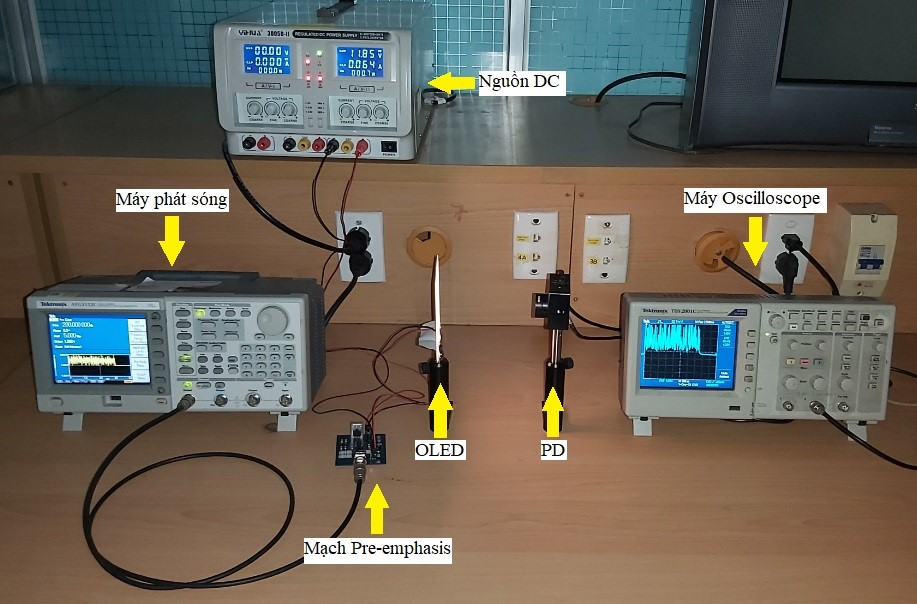
\includegraphics [scale=0.6] {Image/VLC_thucte}
\caption{Hệ thống \ac{vlc} thực tế tại phòng thí nghiệm 209B1}
\end{figure}
\begin{table}[ht]
	\caption{Bảng các thành phần của hệ thống VLC thực tế}.
	\begin{center}
	\small
		\begin{tabular}{|c|c|}
			\hline
			Thiết bị & Thông số\\
			\hline
			\multirow{2}{*}{Generator Tektronik AFG 3152C}
    			&Tốc độ lấy mẫu tối đa 1GS/s, 2 kênh, băng thông 150MHz\\
			&Có thể phát dạng sóng Sine, Square, Pulse, Ramp, Guassian,…. \\			
			&Điều chế AM, FM, PM, FSK, PWM \\
			&Nguồn 100 - 240 V, 47 - 63 Hz\\
			\hline
			\multirow{2}{*}{Oscilloscope Tektronik TDS 2024C}
			&Tốc độ lấy mẫu tối đa 2GS/s\\
			&Băng thông 200MHz\\ 
			&Void/Div tối thiểu 2mV\\
			&4 Channels \\
			\hline
			\multirow{2}{*}{\ac{oled}} \cite{lgN6SA30C} 
			& Băng thông 5KHz\\
			& Kích thước: 100 $\times 100 \times 0.88 mm$\\
			& Công suất tiêu thụ: 1.28 W\\
			& Độ sáng: 75 lm\\
			& Dòng DC: 150 mA\\
			& Điện áp: 8.5 V\\
			\hline
			\multirow{2}{*}{Photodiode (PD)} \cite{APD410A}
			& ADP410A/M của ThorLab \\
			& Bước sóng từ 400 – 1000 nm \\
			& Nguồn: $\pm$ 12 V, 250 mA \\
			\hline
			\multirow{2}{*}{Nguồn DC Yihua 3005D}
			& 0-30 V*2 / 0-5 A*2 \\
			& 2.5 V / 3.3 V / 5 V * 3 A \\
			\hline
		\end{tabular}
		\label{tab:VLC_thucte}
	\end{center}
\end{table}
\paragraph{Điều kiện đo đạc thực tế:}
Hệ thống \ac{vlc} được đặt tại phòng thí nghiệm 209B1, trường Đại học Bách Khoa thành phố Hồ Chí Minh. Nhiệt độ phòng thì nghiệm là $25^o C$, trong điều kiện tắt tất cả các đèn chiếu sáng khác, có ít nguồn sáng tự nhiên từ bên ngoài vào.
\begin{figure}
	\centering
	\begin{subfigure}{.5\textwidth}
		  \centering
		  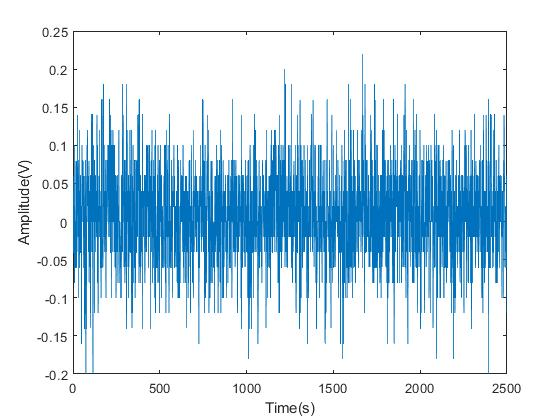
\includegraphics[width=1\linewidth]{Image/floor_noise}
		  \caption{Nhiễu nền trong điều kiện đo đạc của luận văn này}
		  \label{fig: floor_noise}
	\end{subfigure}%
	\begin{subfigure}{.5\textwidth}
		  \centering
		  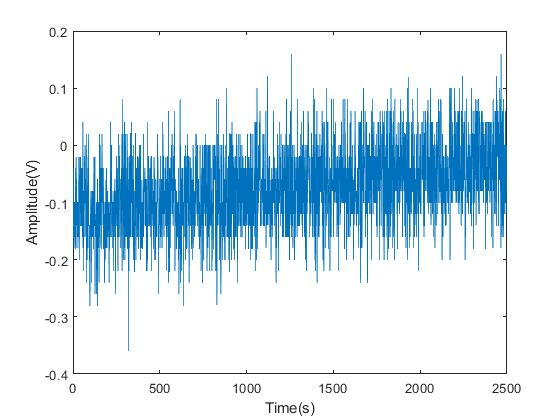
\includegraphics[width=1\linewidth]{Image/fluorescence_noise}
		  \caption{Nhiễu nền trong điều kiện có bật thêm đèn huỳnh quang để chiếu sáng}
		  \label{fig: fluo_noise}
	\end{subfigure}
	\caption{Nhiễu nền trong hai điều kiện}
	\label{fig:noise}
\end{figure}

\begin{figure} [ht]
	\centering
	\captionsetup{justification=centering}
	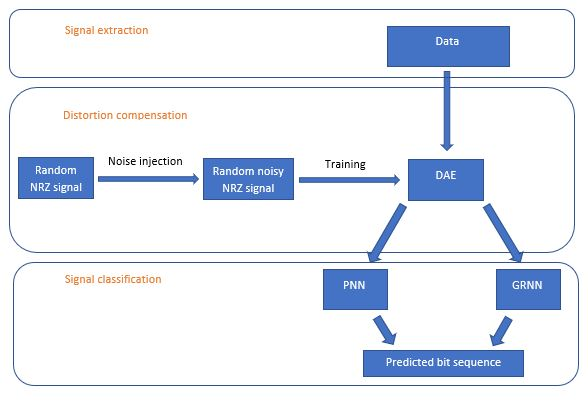
\includegraphics [scale=1] {Image/flow_chart}
	\caption{Sơ đồ khối các phương pháp tiền xử lý và phân loại tín hiệu}
\end{figure}

\subsection{Dữ liệu}
 \paragraph{Tín hiệu phát}
 Để giảm sự thay đổi tín hiệu đột ngột của tín hiệu \ac{nrz}, chúng tôi sử dụng xung Lorentz để thay thế. 
\begin{figure} [ht]
	\centering
	\captionsetup{justification=centering}
	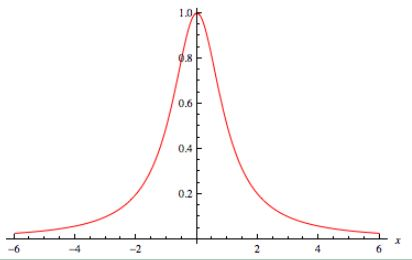
\includegraphics [scale=0.7] {Image/lorentz_pulse}
	\caption{Xung lorentz}
\end{figure}

Hàm Lorentzian với một đỉnh được định nghĩa bởi:

\begin{equation}
L(x) = \frac{1}{\pi}\frac{\frac{1}{2} \Gamma}{{(x-x_0)}^2+ {\frac{1}{2} \Gamma}^2}
\end{equation}
 Trong đó $x_0$ là trung tâm, $\Gamma$ là tham số được đặc trưng bởi chiều rộng có tên là Full Width at Half Maximum. Hàm Lorentz có phân bố xác suất theo phân bố Cauchy. Hàm Lorentz có biến đổi Fourier là 
\begin{equation}
\mathcal{F}[\frac{1}{\pi}\frac{\frac{1}{2}\Gamma}{(x-x_0)^2 + (\frac{1}{2}\Gamma)^2}] =e^{-2\pi i k x_0 - \Gamma \pi |k|.} 
\end{equation}

\paragraph{Trích xuất dữ liệu:}

Tín hiệu truyền đi gồm có 250 ký hiệu, trong đó có 9 ký hiệu pilot dùng để nhận dạng điểm bắt đầu của chuỗi ký hiệu truyền đi. 
Sau khi thu được dữ liệu từ oscilloscope, chuỗi bit truyền đi được trích xuất lại bằng cách so sánh với với chuỗi bit truyền đi thông qua phép tính correlation. 

\begin{figure}
	\centering
	\begin{subfigure}{.5\textwidth}
		  \centering
		  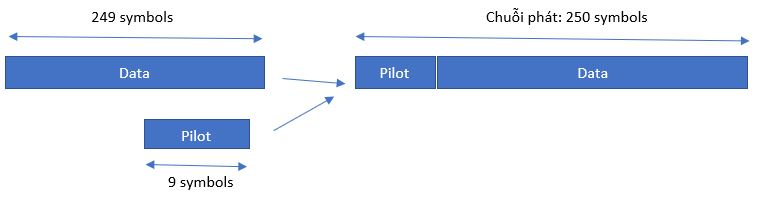
\includegraphics[width=1\linewidth]{Image/data_sequence}
		  \caption{Cấu tạo chuỗi dữ liệu}
	\end{subfigure}%
	\begin{subfigure}{.5\textwidth}
		  \centering
		  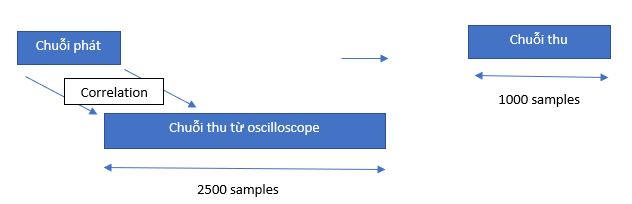
\includegraphics[width=1\linewidth]{Image/data_extracting}
		  \caption{Quá trình trích xuất dữ liệu tại phía thu}
	\end{subfigure}
	\caption{Trích xuất dữ liệu:}
	\label{fig: signal_extraction}
\end{figure}

\paragraph{Phân tích dữ liệu:}

Khi không dùng neural networks, việc giải điều chế sẽ dựa trên một giá trị ngưỡng có thể thay đổi được. Để ước lượng được \ac{snr} của tín hiệu, cần phải tính thông qua giản đồ mắt. Từ giá trị của \ac{snr} có thể tính ra được giá trị của \ac{ber}.

Giá trị \ac{snr} được ước lượng qua công thức:
\begin{equation}
SNR  = \frac {\frac{mean(HighLevel) - mean (LowLevel)}{\sigma(HighLevel) + \sigma(LowLevel)}}{M-1}
\end{equation}
Trong đó: giá trị mức cao và mức thấp được lấy tại thời điểm đồ thị mắt mở rộng nhất. Độ rộng của mắt được tính bằng $(mean(HighLevel) - 3\sigma(HighLevel)) - (mean(LowLevel) + 3\sigma(LowLevel)) $. 

Công thức trên được tính theo Volt, nên cần đổi ra dB bằng cách lấy $20\log_{10}$ kết quả ở trên. 

Có 2 cách để ước lượng \ac{ber} là ước lượng dựa trên \ac{snr} và lấy thương của tổng số bit bị sai và tổng số bit truyền đi. Có thể tính \ac{ber} dựa trên \ac{snr} theo công thức: \cite{Apena_2018}
\begin{equation}
\ac{ber} = \frac{M-1}{M} erfc({\sqrt{\frac{\ac{snr}}{2(M-1)}}})
\end{equation}

\paragraph{Phương pháp đánh giá:} Chất lượng của mô hình được đánh giá thông qua 2 thông số là \ac{snr} và \ac{ber} được tính toán dựa trên 10000 bits thu được (bỏ qua vấn đề đồng bộ ở phía thu và phía phát). Sử dụng kỹ thuật K-fold cross validation để có thể test toàn bộ 10000 bits trên. Dữ liệu được chia ngẫu nhiên thành 5 nhóm, mỗi nhóm 2000 bits, sử dụng 4 nhóm cho việc train và 1 nhóm còn lại cho việc test. Lặp lại cho đến khi test đủ tất cả các nhóm.  

\subsection{Tiền xử lý dữ liệu:}
\paragraph{Framing}
Mỗi symbol đều phụ thuộc vào những symbols đứng trước và sau nó. Vì vậy khi trích dữ liệu để training, chúng ta cần chia dữ liệu thành frame, mỗi frame bao gồm 1 symbol thu được tương ứng với symbol truyền đi cùng với 2 symbols trước và 2 symbols phía sau nó. Như vậy, mỗi frame sẽ bao gồm 5 symbols, các frame liền nhau thì chống lần lên nhau.

\begin{figure} [ht]
	\centering
	\captionsetup{justification=centering}
	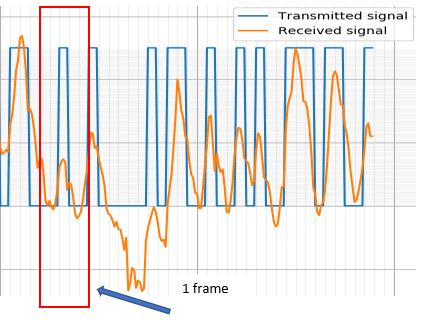
\includegraphics [scale=0.8] {Image/Framing}
	\caption{Cách một frame được trích ra từ tín hiệu thu}
\end{figure}

\paragraph{Đánh giá feature importance bằng Random Forest}
Tại mỗi bit rate, mối quan hệ giữa các symbols và những bit đứng trước và sau nó sẽ có sự khác nhau. Vì vậy, cần một phương pháp có thể đánh giá một cách tương đối mức độ quan trọng của các samples. Trong báo cáo này, chúng tôi sẽ sử dụng Random Forest để đánh giá feature importance.
\begin{figure}
     \centering
     \begin{subfigure}[b]{0.45\textwidth}
         \centering
         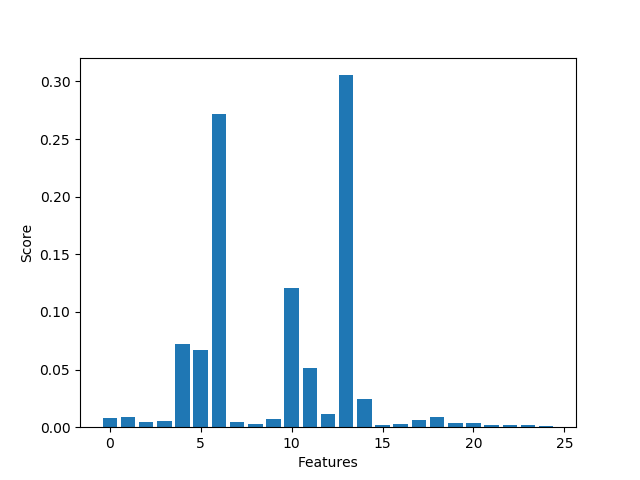
\includegraphics[width=\textwidth]{Image/feature_importance_100k}
         \caption{100kbps}
     \end{subfigure}
     \hfill
     \begin{subfigure}[b]{0.45\textwidth}
         \centering
         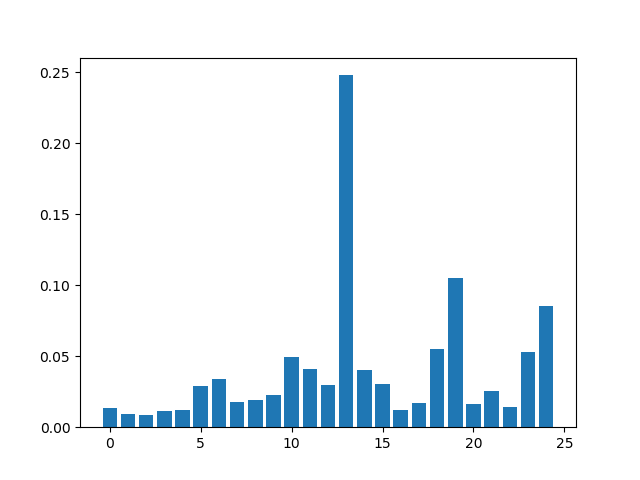
\includegraphics[width=\textwidth]{Image/feature_importance_150k}
         \caption{150kbps}
     \end{subfigure}
     \hfill
     \begin{subfigure}[b]{0.45\textwidth}
         \centering
         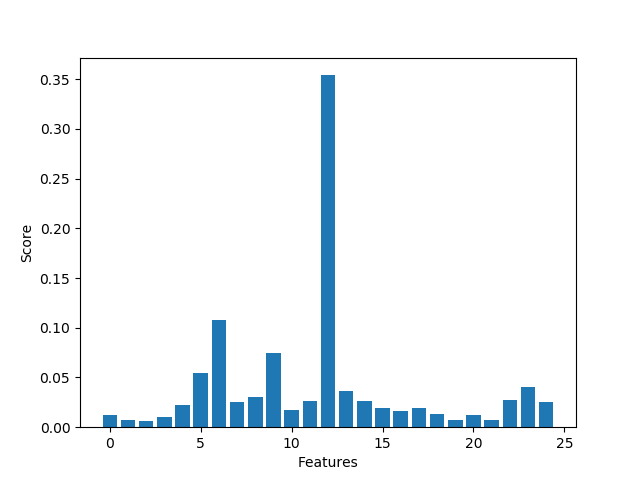
\includegraphics[width=\textwidth]{Image/feature_importance_200k}
         \caption{200kbps}
     \end{subfigure}
          \hfill
     \begin{subfigure}[b]{0.45\textwidth}
         \centering
         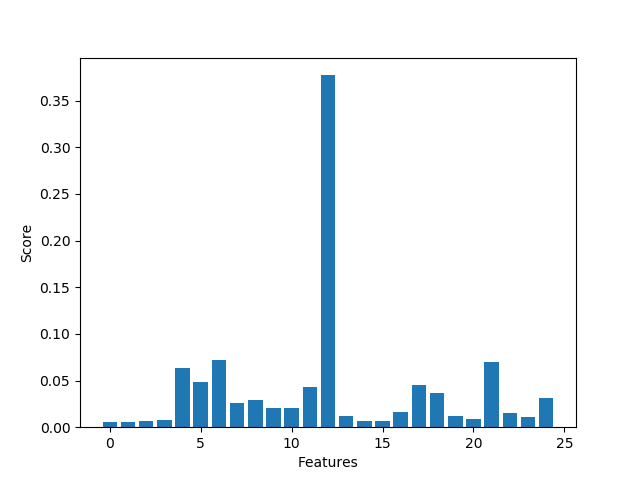
\includegraphics[width=\textwidth]{Image/feature_importance_250k}
         \caption{250kbps}
     \end{subfigure}
        \caption{Đánh giá dữ liệu bằng feature importance}
        \label{fig:feature_importance}
\end{figure}
\paragraph{Áp dụng biến đổi wavelet liên tục}
Mother wavelet được chọn là Mexican hat (richer) vì nó có sự tương đồng nhiều nhất với tín hiệu.
\begin{equation}
\psi(t) = \frac{2}{\sqrt{3} \sqrt[4]{\pi}} \exp^{-\frac{t^2}{2}} \left( 1 - t^2 \right)
\end{equation}
Bề rộng (width) được chọn là 3.
\ac{cwt} chỉ cho kết quả rõ ràng khi tín hiệu có nhiều thông tin hơn. Vì vậy, trong báo cáo này, chúng tôi chỉ áp dụng \ac{cwt} cho trường hợp tín hiệu trước đó đã được tiền xử lý bằng cách lấy theo frame.

\paragraph{Hiệu chỉnh tín hiệu bằng \ac{dae}:}

Như đã trình bày ở chương trước, với giới hạn băng thông điều chế của \ac{oled}, chúng ta phải sử dụng thêm bộ pre-emphasis để làm tăng băng thông. Nhưng cũng chính vì điều này mà méo dạng phi tuyến cũng tăng theo. 
Trong báo cáo này, chúng ta sẽ tập trung vào việc làm giảm sự méo dạng phi tuyến của \ac{oled} bằng bộ bù post-distortion. 

Ngõ vào của mô hình là tín hiệu cùng loại với tín hiệu trước khi qua kênh truyền \ac{vlc}. Mô hình sẽ học theo kiểu unsupervised learning, nghĩa là chỉ học những đặc tính của tín hiệu trước khi qua kênh truyền mà không cần phải dán nhãn. Tín hiệu sử dụng trong hệ thống \ac{vlc} rất đơn giản nên việc bị overfitting là không thể tránh khỏi. Để giảm thiểu overfitting có thể sử dụng kỹ thuật noise injection để tăng độ phức tạm cho dữ liệu đầu vào. 

Để tạo ra dữ liệu để train cho mô hình \ac{dae}, chúng ta cần tạo ra một chuỗi tín hiệu ngẫu nhiên có số lượng mẫu bằng với dữ liệu cần hiệu chỉnh. Ví tín hiệu tạo ra được rất đơn giản nên mô hình sẽ rất dễ bị overfitting, để giảm thiểu tình trạng này, cần áp dụng kỹ thuật noise injection để tăng độ phức tạp cho tín hiệu.

Như vậy, mô hình \ac{dae} sẽ sử dụng tín hiệu sau khi thêm nhiễu để học mà không cần dán nhãn cho tín hiệu. Mô hình sẽ học những đặc trưng của tín hiệu 2 mức khi không bị méo dạng. 
Sau khi mô hình \ac{dae} được training xong, tín hiệu ngõ ra của hệ thống \ac{vlc} sẽ được đưa vào để có thể hiệu chỉnh lại tín hiệu bị méo dạng. (Vì nhiễu là ngẫu nhiên nên chất lượng của mô hình qua mỗi lần train sẽ cho kết quả có đôi chút khác biệt).

Để tăng hiệu quả cho mô hình \ac{dae}, chúng tôi xây dựng các layer dựa trên mô hình \ac{lstm}. \ac{lstm} sẽ giúp mô hình \ac{dae} có thể học được những đặc điểm, mối quan hệ của những bit liền kề. (trong báo cáo này, chúng tôi sẽ không đề cập về cơ sở lý thuyết \ac{lstm}).
Một số thông số cho mô hình \ac{dae} như:
\begin{itemize}
\item Optimizer: Stochastic Gradient Descent with mini batch
\item Learning rate: 0.001
\item Epoch: 100
\end{itemize}

\begin{figure}
	\centering
	\begin{subfigure}{.45\textwidth}
		  \centering
		  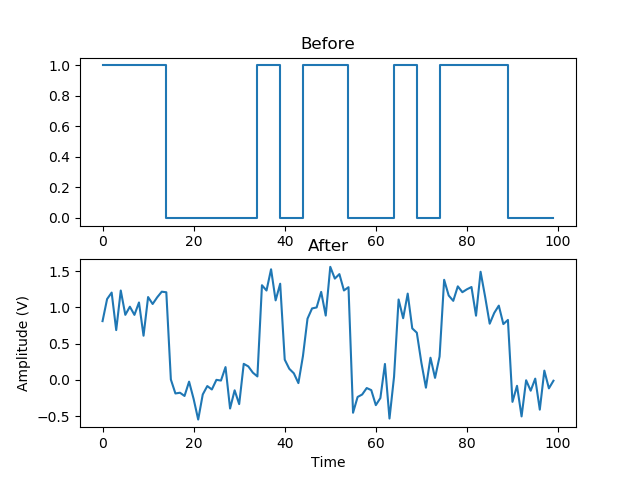
\includegraphics[width=1\linewidth]{Image/dae_noise_injection}
		  \caption{Tín hiệu trước và sau khi thêm nhiễu (dùng cho training)}
		  \label{fig: floor_noise}
	\end{subfigure}
	\begin{subfigure}{.45\textwidth}
		  \centering
		  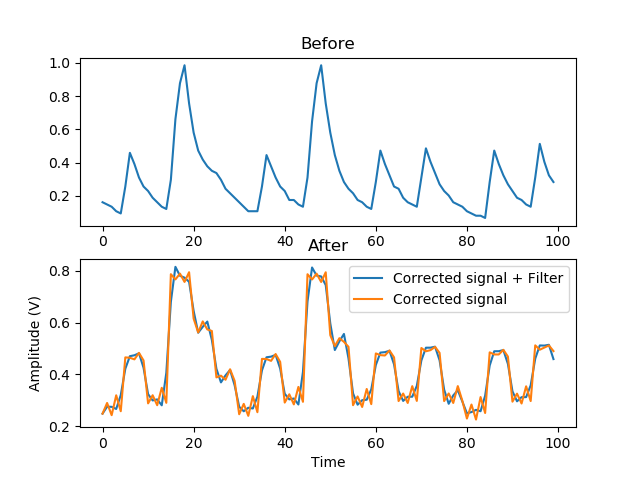
\includegraphics[width=1\linewidth]{Image/corrected_signal}
		  \caption{Tín hiệu ngõ ra của hệ thống \ac{vlc} trước và sau khi được hiệu chỉnh}
		  \label{fig: fluo_noise}
	\end{subfigure}
	\caption{Mô hình \ac{dae}}
	\label{fig:dae}
\end{figure}

Tín hiệu sau khi đi qua mô hình \ac{dae} sẽ có khá nhiều nhiễu, vì vậy nó cần được đi qua thêm một bộ lọc để giảm bớt nhiễu. Có thể thấy tín hiệu sau khi đi qua \ac{dae} và bộ lọc có chất lượng tốt hơn nhiều so với tín hiệu ban đầu. Các mức của tín hiệu có thể dể dàng phân biệt được, như vậy là đã làm giảm đáng kể tình trạng méo dạng của tín hiệu.

\section{Kết quả và phân tích}
\subsection{Khảo sát tín hiệu:} 
Trong phần này, chúng tôi sẽ tiến hành khảo sát tín hiệu tại các tốc độ bit khác nhau để tìm ra tốc độ bit phù hợp để phân tích và so sánh tín hiệu \ac{nrz} với tín hiệu xung Lorentz. Để thấy hiệu quả của các phương pháp tiền xử lý, phân loại cũng như việc sử dụng xung Lorentz, chúng tôi sẽ so sánh các phương pháp này với nhau và với kết quả của những nghiên cứu trước đó cũng tại trường đại học Bách Khoa TP. HCM với cùng một hệ thống \ac{vlc}. Trong đó, sử dụng điều chế \ac{nrz} 2 mức, phân loại bằng \ac{pnn}, không qua tiền xử lý. Tốc độ tối đa đạt được là 25kbps khi ước lượng \ac{ber} thông qua \ac{snr} và 53kbps khi dùng \ac{pnn} để phân loại.

Để thấy hiệu quả của các phương pháp tiền xử lý, phân loại cũng như việc sử dụng xung Lorentz, chúng tôi sẽ so sánh các phương pháp này với nhau và với kết quả của những nghiên cứu trước đó cũng tại trường đại học Bách Khoa TP. HCM với cùng một hệ thống \ac{vlc}. Trong đó, sử dụng điều chế \ac{nrz} 2 mức, phân loại bằng \ac{pnn}, không qua tiền xử lý. Tốc độ tối đa đạt được là 25kbps khi ước lượng \ac{ber} thông qua \ac{snr} và 53kbps khi dùng \ac{pnn} để phân loại (không qua tiền xử lý).

\begin{figure} [ht]
	\centering
	\captionsetup{justification=centering}
	\includegraphics [scale=0.8] {Image/BER_20cm}
	\caption{\ac{ber} ước lượng tại các tốc độ bit khác nhau khi dùng xung Lorentz}
	\label{fig:BER_20cm}
\end{figure}
Hình \ref{fig:BER_20cm} cho thấy, nhìn chung việc dùng tín hiệu xung Lorentz ngõ vào làm cho tín hiệu ngõ ra khó nhận dạng hơn bằng cách ước lượng \ac{ber} thông qua \ac{snr}, không có tốc độ bit nào đạt ngưỡng khi dùng Lorentz. Tuy nhiên nó lại giúp mạch đáp ứng tốt hơn, vẫn có thể phân biệt bằng mắt khi tốc độ vượt quá 70kbps, trong khi đó tín hiệu \ac{nrz} thì không còn phân biệt được nữa.
 
\subsection{Phân loại các mức tín hiệu:}

Hai mô hình được sử dụng trong báo cáo này là \ac{pnn} và \ac{grnn}, cả hai mô hình trên đều được phát triển bởi Specht và đều là mô hình one-pass. Với lợi thế là về mặt tốc độ cũng như khả năng chống chịu nhiễu. Để thể hiện được hiệu quả của 2 mô hình trên, chúng tôi sẽ về \ac{ber} và thời gian (thực hiện trên Google Colab).

Độ lệch chuẩn được chọn cho phương pháp \ac{pnn} khi chỉ lấy một symbol khá nhỏ (từ 0.05 đến 0.3) và tăng dần khi tăng khoảng cách. Đối với \ac{grnn}, độ lệch chuẩn lớn hơn nhiều lần so với \ac{pnn} (từ 3 đến 7), và cần giảm dần khi tăng khoảng cách. Đối với trường hợp sử dụng \ac{dae}, độ lệch chuẩn cần nhỏ hơn từ 5 đến 10 lần với \ac{pnn} và lớn hơn từ 5 đến 10 lần với \ac{grnn}.

\begin{table}[ht]
	\caption{Bảng so sánh độ chính xác của các phương pháp khi chỉ lấy một symbol}.
	\begin{center}
	\small
		\begin{tabular}{|c|c|c|c|c|}
			\hline 
			\backslashbox{Phương pháp}{Khoảng cách(cm) } & 10& 20 & 30 & 40\\
			\hline
			Không dùng neural networks & 0.1928 & 0.2077 & 0.2006 & 0.2194\\
			\hline 
			\ac{pnn} & 0.1377 & 0.1867 & 0.1744 & 0.2089\\
			\hline
			\ac{grnn} & 0.1394 & 0.1861 & 0.1745 & 0.2090\\
			\hline
			\ac{pnn} + \ac{dae} & 0.0356 & 0.0544 & 0.0585 & 0.0999\\
			\hline
			\ac{grnn} + \ac{dae} & 0.0347 & 0.0053 & 0.0566 & 0.0910\\
			\hline
		\end{tabular}
		\label{tab:result_1}
	\end{center}
\end{table}

Khi lấy dữ liệu theo frame và áp dụng \ac{cwt}, cần chọn độ lệch chuẩn trong hai phương pháp là \ac{pnn} và \ac{grnn} cao hơn so với không dùng \ac{cwt}, thông thường là gấp đôi.
\begin{table}[ht]
	\caption{Bảng so sánh độ chính xác của các phương pháp khi lấy một frame}.
	\begin{center}
	\small
		\begin{tabular}{|c|c|c|c|c|}
			\hline 
			\backslashbox{Phương pháp}{Khoảng cách(cm) } & 10& 20 & 30 &40\\
			\hline
			\ac{pnn} & 0.0065 & 0.0096 & 0.0125 & 0.0321\\
			\hline
			\ac{grnn} & 0.0064 & 0.0095 & 0.0127 & 0.0311\\
			\hline
			\ac{pnn} + \ac{cwt} & 0.0065 & 0.0085 & 0.0118 & 0.0341\\
			\hline
			\ac{grnn} + \ac{cwt} & 0.0067 & 0.0088 & 0.0119 & 0.0338\\
			\hline 
			\ac{dtnn} & 0.0052 & 0.0087 & 0.0126 & 0.0317\\
			\hline
		\end{tabular}
		\label{tab:result_2}
	\end{center}
\end{table}

Từ kết quả thu được như trên, có thể thấy việc dùng \ac{dae} để bù méo dạng đem lại hiệu quả tốt nhất khi chỉ dùng một symbol để phân loại. Trong khi đó, framing mang lại hiệu quả đáng kể cho việc nhận dạng. Từ đó, ý tưởng của chúng tôi là kết hợp hai loại dữ liệu này lại với nhau và mô hình \ac{dtnn} là lựa chọn vô cùng phù hợp trong trường hợp này.

\begin{table}[ht]
	\caption{Bảng so sánh thời gian train và test các phương pháp}
	\begin{center}
	\small
		\begin{tabular}{|c|c|c|c|}
			\hline 
			Phương pháp & Thời gian train (s) & Thời gian test (s)\\
			\hline 
			\ac{pnn} & - & 4.63 \\
			\hline
			\ac{grnn} & - & 19.53\\
			\hline
			\ac{dae} & 103.25 & 1.9291 \\
			\hline
			\ac{pnn} + Framing & - & 12.18 \\
			\hline
			\ac{grnn} + Framing & - & 35.11 \\
			\hline
			\ac{pnn} + \ac{cwt} & - & 47.37 \\
			\hline
			\ac{grnn} + \ac{cwt} & - & 86.22 \\
			\hline
			\ac{dtnn} & - & 63.51 \\
			\hline
		\end{tabular}
		\label{tab:time}
	\end{center}
\end{table}
Thời gian train và test của các phương pháp được thể hiện trong bảng \ref{tab:time}, trong đó kết quả test trên Google Colab. Chỉ có mô hình \ac{dae} là có thể lưu lại mô hình và sử dụng cho nhiều bit rate và khoảng cách khác nhau. Vì sử dụng K-fold validation để đánh giá dữ liệu nên không thể lưu lại mô hình cho \ac{dtnn} mà phải train lại cho mỗi lần cần test. Trong trường hợp có đủ dữ liệu (lớn hơn 20000 bits), có thể lưu lại mô hình \ac{dtnn}, từ đó thời gian test có thể giảm đi khoảng 3-4 lần. 

\section{Kết luận chương}
Trong báo cáo này, chúng tôi đã xây dựng các mô hình có khả năng phân loại các mức tín hiệu và các mô hình để tiền xử lý cho tín hiệu. Để thấy được sự hiệu quả, chúng tôi đã so sánh các phương pháp này với nhau và với kết quả từ nghiên cứu trước đó.

Đầu tiên, chúng ta sẽ đi so sánh các phương pháp tiền xử lý tín hiệu. Từ bảng \ref{tab:result_1} có thể thấy việc phân loại tín hiệu bằng neural networks (không qua tiền xử lý) vẫn đem lại hiệu quả đôi chút so với khi không dùng. Tuy nhiên sai số vẫn còn rất lớn và không thể ứng dụng cho mô hình thực tế. Sau đó, sau khi dùng thêm \ac{dae} để hiệu chỉnh tín hiệu \ac{ber} đã giảm đáng kể, giảm 4 lần. Mặc dù vậy, \ac{ber} vẫn còn khá cao, chưa thể áp dụng vào hệ thống \ac{vlc} được. Việc hiệu quả của \ac{dae} chưa cao như kỳ vọng là do ngay từ đầu tín hiệu truyền đi không phải là xung vuông, trong khi đó nhiệm vụ của \ac{dae} là đưa tín hiệu về càng giống tín hiệu \ac{nrz} càng tốt.

Nhận thấy các bit liền kề có sự liên hệ với nhau, chúng tôi đã ứng dụng một kỹ thuật của xử lý tiếng nói là Framing để tăng độ chính xác cho mô hình. Từ bảng \ref{tab:result_2}, có thể thấy Framing giúp \ac{ber} giảm đi 20 lần xuống dưới mức 0.01 tại các khoảng cách 10 và 20 cm. Ngoài ra, chúng tôi còn áp dụng thêm một kỹ thuật khác là \ac{cwt}, kết quả cho thấy \ac{ber} giảm đi đôi chút. Từ kết quả của Framing và \ac{dae}, chúng tôi đã sử dụng \ac{dtnn} để giảm \ac{ber}, kết quả là \ac{dtnn} cũng giúp giảm \ac{ber}, đặc biệt là ở 10 cm.

Kế đến, chúng tôi sẽ so sánh 3 phương pháp được sử dụng trong luận văn là \ac{pnn}, \ac{grnn} và \ac{dtnn}. Từ ba bảng \ref{tab:result_1}, \ref{tab:result_2} và \ref{tab:time} cho thấy \ac{pnn} và \ac{grnn} mang lại hiệu quả tương đối ngang nhau, \ac{dtnn} thì nhỉnh hơn đôi chút. Tuy nhiên, thời gian chính là ưu thế rất lớn của \ac{pnn} so với hai phương pháp còn lại. Ngoài ra, xét về tính khả thi khi triển khai mô hình thực tế, \ac{pnn} và \ac{grnn} cũng chiếm phần lợi thế hơn so với \ac{dtnn} vì chỉ sử dụng các phép tính toàn đơn giản, hoàn toàn có thể lập trình bằng C/C++ trên những vi xử lý giá rẻ, không cần lập trình Python trên các vi xử lý đắt tiền hơn như \ac{dtnn}.

Tóm lại, qua khảo sát ở trên có thể thấy xung Lorentz làm tín hiệu trở nên khó phân loại hơn so với \ac{nrz}. Tuy nhiên, nó lại giúp mạch đáp ứng tốt hơn. Từ đó, khi kết hợp Lorentz cùng với những phương pháp mạnh mẽ hơn có thể mang lại hiệu quả đáng kể. Khảo sát của chúng tôi cho thấy, phương pháp của chúng tôi có thể giúp bit rate tăng 4 lần so với phương pháp truyền thống và tăng gần 2 lần so với khi áp dụng tín hiệu \ac{nrz} cùng với những phương pháp xử lý đơn giản.
\chapter{Kết luận}\label{sec:chapter_4}
\section{Tóm tắt và kết luận chung}

\subsection{Ưu điểm}
\begin{itemize}
\item Xây dựng thành công 3 mô hình có thể phân loại được 2 mức của tín hiệu.
\item So sánh 2 phương pháp phân loại tín hiệu là \ac{pnn} và \ac{grnn} với phương pháp thường được sử dụng là \ac{cnn}
\item Xây dựng mô hình có khả năng cải thiện tín hiệu bị méo dạng.
\item Đề xuất phương pháp xử lý tín hiệu bằng cách tách dữ liệu theo frame.
\item Đề xuất sử dụng xung Lorentz thay thế cho tín hiệu \ac{nrz}.
\end{itemize}

\subsection{Nhược điểm}
\begin{itemize}
\item Tín hiệu chỉ có 2 mức
\item Số tốc độ bit và khoảng cách được khảo sát ít. 
\end{itemize}
\subsection{Nguyên nhân chưa đạt}
\begin{itemize}
\item Chưa giành đủ thời gian nghiên cứu, thí nghiệm.
\item Chưa có đủ kiến thức về generative model.
\end{itemize}

\subsection{Cách khắc phục}
\begin{itemize}
\item Khảo sát thêm các nhiều tốc độ bit ở những khoảng cách khác nhau.
\item Học tập và nghiên cứu sâu về AI và generative model.
\item Thay đổi mạch lái \ac{oled}
\end{itemize}

\section{Hướng phát triển}
\begin{itemize}
\item Xây dựng mô hình bù méo dạng tốt hơn: có thể ứng dụng những phương pháp như \ac{gan}, Adversarial Denoising Autoencoder, ...
\item Kết hợp sức mạch của nhiều mô hình lại với nhau thông qua mô hình Stacking. 
\item Phát triển hệ thống thành MINO
\item Thiết kế mạch lái \ac{oled} phù hợp.
\end{itemize}
\bibliographystyle{reference/IEEEtran}
\bibliography{IEEEabrv,reference/tailieuthamkhao}
\hfill
\chapter*{Phụ lục}
\paragraph{Ngôn ngữ lập trình:} Python, Matlab.
\paragraph{Thư viện Python hỗ trợ:}
\begin{itemize}
\item Tensorflow (2.4.1)
\item Keras (2.2.5)
\item Matplotlib (3.1.0)
\item Numpy (1.19.5)
\item Pandas (0.24.2)
\item Statsmodels (0.11.1)
\item Scikit learn (0.23.1)
\item Scipy (1.5.2)
\item Pywavelet (1.1.1)
\item Streamlit (0.75.0)
\end{itemize}
\paragraph{Code:}
\href{https://drive.google.com/drive/folders/129JB8ezu-k2oR61VSAxTXn42dlDtAsw5?usp=sharing}{Google Drive}
Hoặc
\href{https://github.com/hieunguyen810/Web-app-VLC-system}{Github}

Ghi chú:
\begin{itemize}
\item Configure.json: Cấu hình các phương pháp xử lý, khoảng cách, bitrate, mô hình, ...
\item Main.py: file thực thi chính cho chương trình
\item Getdata.py: trích xuất và xử lý dữ liệu
\item Model.py: lưu trữ các mô hình như \ac{pnn}, \ac{grnn}, \ac{dtnn}, \ac{dae}.
\end{itemize}
Hướng dẫn sử dụng chi tiết (readme.txt) cũng như các file configure.json, default-std-PNN.json, default-std-GRNN.json có thể được tìm thấy tại các đường dẫn phía trên. 
\begin{figure} [ht]
	\centering
	\captionsetup{justification=centering}
	\includegraphics [scale=0.7] {Image/sample_results}
	\caption{Kết quả thu được}
	\label{fig:BER_20cm}
\end{figure}

\small
$Main.py$
\lstinputlisting[language=Python, numbers=left, breaklines]{Code/Main.py}
$Model.py$
\lstinputlisting[language=Python, numbers=left, breaklines]{Code/Model.py}
$Getdata.py$
\lstinputlisting[language=Python, numbers=left, breaklines]{Code/Getdata.py}
\end{document}